\documentclass[12pt,a4paper]{report}
%% Packages élémentaires %%
\usepackage[utf8]{inputenc}
\usepackage{mathpazo,etoolbox, graphicx, wrapfig, pbox, fancybox, hyperref, appendix, geometry, amsmath, amssymb, tikz, pgfplots, calc, enumitem}
\graphicspath{{images/}}
\geometry{hmargin=2.4cm, vmargin = 2.1cm}
\setlist[itemize]{itemsep=10pt, label={--}}

%% Couleurs %%
\usepackage{xcolor}
\definecolor{bleu}{RGB}{14, 68, 175}
\definecolor{bleu3}{RGB}{222, 233, 255 }
\definecolor{orange2}{RGB}{255, 216, 154}
\definecolor{rouge}{RGB}{201, 0, 0}
\definecolor{vert}{RGB}{14, 137, 0}
\definecolor{gris}{RGB}{222,230,230}
\newcommand\rouge[1] {{\color{rouge}{#1}}}
\newcommand\bleu[1] {{\color{bleu}{#1}}}
\newcommand\green[1]{{\color{vert}{#1}}}


%% Cadres %%
\newcommand\bb[1]{
\begin{center}
\fcolorbox{black}{bleu3}{\parbox{\textwidth}{ 
#1
}}
\end{center}}

\newcommand\boite[1]{
\begin{center}
\fbox{\parbox{\textwidth}{ \begin{center}
\begin{Large}
#1
\end{Large}
\end{center}}}
\end{center}}

\newcommand\aparte[1]{
\begin{center}
\fcolorbox{white}{gris}{\parbox{\linewidth}{ \textit{A parte} \\
#1 }}
\end{center}}

\newcommand\exemple[1]{
\begin{center}
\fcolorbox{white}{gris}{\parbox{\linewidth}{ \textit{Exemple} \\
#1 }}
\end{center}}

%% Commandes %%
\newcommand\imp[1]{\underline{\textbf{#1}}}
\newcommand\eq[1]{\begin{large}
\begin{align*}
#1
\end{align*}
\end{large}}
%% Commandes fantaisistes (cf. Internet) %%
\renewcommand{\parallel}{ \mathbin{\!/\mkern-5mu/\!} }
\newcommand{\q}[1]{{%
\font\larm = larm1000%
\larm%
\char 190}{ \textit{#1} }{%
\font\larm = larm1000%
\larm%
\char 191}}

%% Wrapping %%
\newcommand\wrap[4]{\begin{wrapfigure}[#1]{#2}{#3\textwidth}
#4
\end{wrapfigure}}

\usepackage[french]{babel}
\usepackage{times, tikz, calc, enumitem}
\usetikzlibrary{intersections, calc,shapes}
\xdef\Rad{2}
\newcommand{\ARW}[3][]{%
    \foreach \ang in {#2}{%
        \draw[#1] #3 + (\ang:\Rad)--++(\ang+1:\Rad) ;
    }
}
\documentname{Synthèse : Fondements de l'informatique}{B2-IRCI : INFO-H2001 -- Pr. \textsc{Bersini}}{info-garde_v2}
\author{Sami \textsc{Abdul Sater}}
\date{\hspace{-0.6cm}Année académique 2019-2020}
\begin{document}
\newgeometry{margin=1.1cm, lmargin=1.4cm, top=0cm}
%%begin novalidate
\pretitle{\begin{flushleft} \fontsize{30}{34}\selectfont}
\posttitle{\end{flushleft}}
\preauthor{\begin{flushleft} \linespread{1.4} \large}
\postauthor{\end{flushleft}}
\predate{} % remove extra space
\postdate{} % remove extra space
%%end novalidate

\maketitle
\vfill


\thispagestyle{empty}
\restoregeometry
\tableofcontents
\chapter{L'information binaire}
L'informatique et l'information, c'est la même racine, c'est pas moi qui le dit c'est écrit dans mon livre hein 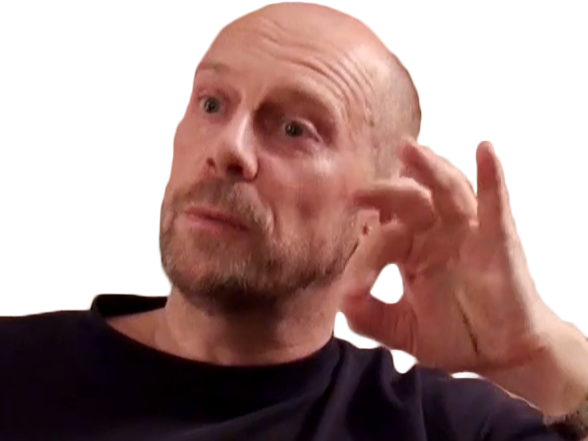
\includegraphics[scale=0.2]{soral}. Si l'on s'intéresse à faire fonctionner une machine qui réalise des instructions, on peut partir de la machine de Turing, la mère du concept même d'ordinateur, pour se rendre compte que l'\underline{information}, dans sa globalité, doit se transférer, se manipuler, etc. Une manière très économe de traiter de l'information pour une machine est le \textbf{binaire} : économe sur les plans fonctionnel et financier -- on ne va pas commencer à distinguer des nuances de "oui" ou de "non". C'est blanc ou noir un point c'est tout. Et un élément d'information binaire est appelé un \textbf{bit}. En pratique, on peut s'imaginer un circuit électronique qui réagit différemment s'il est traversé par du courant ou pas. Ces éléments \textit{logiques}, qui selon le contexte, font passer ou non le courant sont des \textbf{transistors}.
\section{Le transistors et les circuits logiques}
\wrap{20}{r}{0.5}{
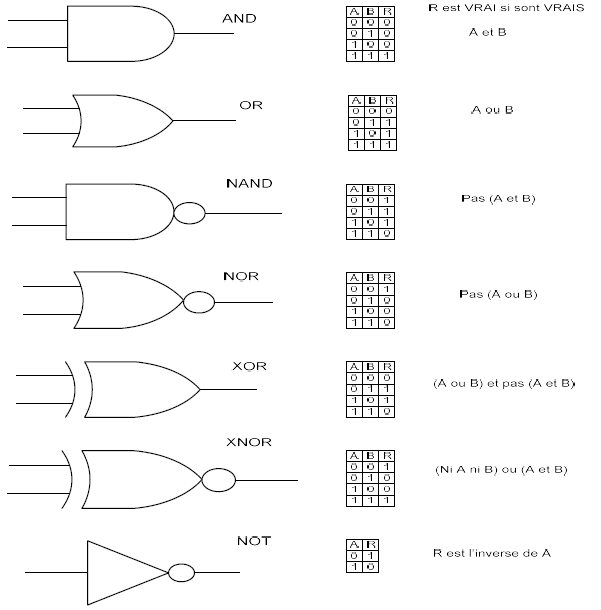
\includegraphics[width=\linewidth]{info-logique}
\centering
\caption{Résumé des schémas logiques.}
\label{fig:circuitLogique}}
Les transistors sont des éléments de circuits électroniques qui permettent sur le plan conceptuel d'effectuer des étapes élémentaires de logique, telles que le "\textbf{et}" et le "\textbf{ou}". Pratiquement ça se traduit par une porte qui laisse passer un courant (ou autre type de signal) ou non. Le nombre de transistors  sur un circuit définit le nombre d'instructions possibles par seconde, et son évolution est prédite à travers la \textit{Loi de Moore}. On arrive petit à petit à saturation, car les transistors deviennent tellement petits (dizaines de nm d'épaisseur) que les électrons peuvent passer à un autre circuit par effet tunnel : on est obligé d'imposer une limite physique à la disposition de transistors.\\
\\
Les circuits logiques permettent de concrétiser en pratique certains concepts logiques, tels que le "ou", le "et", leur négation respective, et autres fumisteries en tout genre dont voici un résumé sur la figure \textbf{\ref{fig:circuitLogique}}.

\subsection{Circuits électroniques}
Les transistors ne sont rien de plus que des composants électroniques auxquels on accorde du sens logique, un peu comme une inductance à laquelle on accorde du sens physique, hein, remember : $$ V = L \dfrac{dI}{dt} \; .$$ Of course ceci n'avait comme seul objectif d'ajouter une équation à une synthèse avec littéralement $\underline{0}$ équations, ou 1, ou 10. L'usage le plus simple des transistors est la disposition en \textbf{série} ou en \textbf{parallèle} dans un circuit.
\begin{description}[leftmargin = !, labelwidth = \widthof{\bfseries Parall. : }]
\item[Série : ] Si l'un des deux transistors empêche le courant de passer, le courant s'arrête dans le circuit : c'est une porte \textit{AND}, il faut que les \textit{DEUX} conditions (les deux transistors) soient validées.
\item[Parall. : ] Si une des deux conditions est validée, alors le courant passe : c'est une porte \textit{OR}.
\end{description}
\subsection{Mémoire électronique}
\wrap{11}{r}{0.3}{\centering 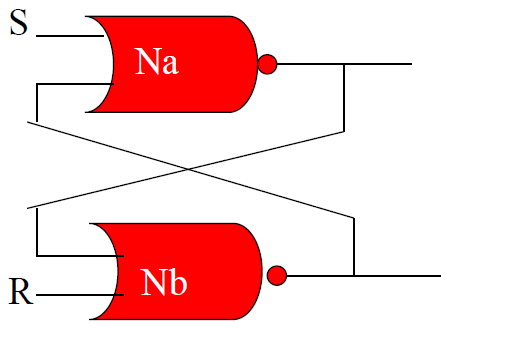
\includegraphics[width=0.9\linewidth]{info-bistable}
\caption{Schéma d'un circuit "bistable"}
\label{fig:bistable}}
L'information circule et est dirigée grâce à des transistors, mais il faut une manière de stocker de l'information. Ceci se fait à l'aide d'un circuit \textbf{bistable} : un circuit possédant deux états stables et capable de passer sur commande de l'un à l'autre. De plus, rappelons que "mémoriser de l'information" ça veut techniquement dire "mémoriser un bit", donc garder la valeur "1" de côté. Okéé, une fois ceci à l'esprit, on regarde le schéma d'une bistable : deux portes \textit{NOR} (cf. figure \textbf{\ref{fig:circuitLogique}}) en parallèle, une avec la fonction "Set" ($\rightarrow$ "S") et l'autre "Reset" ($\rightarrow$ "R"). Pour sauvegarder un bit, on met "S" à 1. Ce faisant, la sortie $Na$ sera à 0, et considérant que "R" est à 0 (parce qu'on ne reset pas), la sortie Nb sera \textit{NOR}$[0,0] = 1$, et voilà, le bit est mémorisé. Si "S" tombe à zéro, Na sera \textit{NOR}$[0,1] =0$ qui, injecté dans la deuxième \textit{NOR} donnera toujours 1.\\
\\
On peut répéter un circuit bistable pour mémoriser 4 bits par exemple (assemblage de 4 bistables). Monsieur Bersini ajoute qu'on peut donc en réalité construire un ordinateur avec un seul type de porte logique : la porte \textit{NOR} ; en quantité... comment dire... beaucoup. \\
\\
De nos jours, les progrès en recherches proposent des basculements (= passer de 0 à 1 pour l'état d'une bistable) grâce à des transitions électromagnétiques, beaucoup plus rapides qu'un électron issou.

\section{L'information binarisée}
Dès lors qu'on a adopté le principe du binaire pour des raisons d'économie, de facilité, et d'universalité, toute chose est transformée en une succession de \textbf{bits} : instructions de programmes, textes, nombres, images, sons, ... Les informaticiens aiment réserver des champs de longueur déterminée pour accueillir chaque donnée. À chaque type de donnée correspond une \underline{codification} symbolique précise. À titre d'exemple, si on ouvre un fichier .txt avec une application censée recevoir des images, ben on va pas avoir un texte smooth.
\subsection{Données logiques}
Les "données logiques" sont les fameux "0 ou 1" qui nous permettent de représenter les données.
\subsubsection{Caractères alphabétiques}
Le standard ASCII propose la représentation des caractères alphabétiques sur 8 bits, soit un \textbf{octet}. UTF-8 aussi.
\subsubsection{Nombres, leur signe, et la représentation en virgule flottante}
Les nombres sont donc codés aussi en bits, et leur signe doit être précisé. Je ne vais pas reprendre l'écriture en base 2, mais je vais introduire le fait que les signes sont inclus dans l'écriture binaire. Faites ce que vous voulez de cette information, j'ai juste la flemme. La représentation en virgule flottante aussi, et pareil.
\subsection{Les images et les films}
Une image est souvent impossible à recoder sous forme vectorielle. Qu'est-ce que la forme vectorielle ? C'est simple. Zoomez \textbf{ici}, jusqu'au maximum. C'est smooth, c'est encré dans le document, c'est vectoriel. En revanche, zoomez là dessus : 
\includegraphics[scale=0.2]{musk}, hmhm c'est pas très quali, c'est pas vectoriel. Vectoriel nécessite une grande précision et un grand taux de \textit{smootherie} ce qui est souvent impossible en pratique. Ce qu'on préfère faire c'est découper une image en une superposition de carrés (=pixels), en gros faire un quadrillage, et la netteté de l'image dépendra de la densité du quadrillage, voilà. Chaque carré a une couleur et une luminosité. Le tout est indiqué en $256^3$ valeurs, soit $3 \times 8$ bits.\\
\\
Avec un petit calcul, on se rend compte que coder un film de quelques heures résulte en une quantité astronomique de données à coder, environ 80 Go. Il faut donc compresser !
\subsection{Regroupement et compression de données}
Alors il faut savoir une chose : on s'intéresse rarement aux bits pris isolément, on les prend souvent en groupe. Par exemple, par 8 : un \underline{octet}. D'autres standards peuvent naitre, comme par exemple la notation \textit{hexadécimale}. En gros, comme on a tendance à des fois manipuler des demi-octets = $4$ bits = $16$ valeurs, on voit l'intérêt de cette notation. La notation se fait à travers des symboles : les 10 chiffres classiques et puis les lettres majuscules, de A à F. Chaque demi-octet est noté par un symbole hexadécimal. La beauté est là :
$$00110100011110111000 \qquad \Longrightarrow \qquad \text{347B8}\; .$$

\subsubsection{Correction d'erreurs de transfert}
Pour garantir la fidélité de l'information échangée, il est préférable de la transférer par des groupes de bits de taille fixe. Pour détecter les erreurs, on adjoint à un octet deux copies additionnelles, formant un total de 3 octets identiques. Pour éviter qu'une erreur se produise, ce qui est encore mieux, on adjoint à l'octet 2 bits supplémentaires, pour pouvoir substituer les combinaisons de 8 bits qui présentent des risques d'erreurs de transmission par des combinaisons plus robustes. À l'arrivée, l'octet est déshabillé et retrouve sa longueur initiale.
\subsubsection{Compression et compaction des données}
\begin{description}[leftmargin=!,labelwidth=\widthof{\bfseries Compression b}]
\item[Compression] Simplification des bits redondants, aucune détérioration de la qualité. Totalement réversible.
\item[Compactage] Allègement le codage des données avec une dépréciation de la qualité. Processus irréversible. Par exemple : recoder une image sur une palette de couleur plus limitée. Un fichier compacté devient inexploitable sans son mode d'emploi !
\end{description}
\subsection{Cryptage des données}
Le cryptage se fait en deux temps : le cryptage et le décryptage. Le cryptage consiste en une modification des données selon un certain algorithme, qu'on peut décoder à l'aide d'une clé de décryptage. Elle est souvent envoyée avec le fichier, sinon c'est vraiment po cool.
%%%%
\chapter{Unité centrale : le processeur}
\aparte{
Good evening Ladies and Gentlemen. J'ai 20 minutes avant que la mise à jour de Warzone se termine, 32Go c'est beaucoup sa grand-mère la nymphe. Je sais pas si toi qui lis cette synthèse (si elle est finie inshallah) tu te demandes dans quel but j'écris ça, mais c'est simple : j'écris ça pour rire quand je vais relire cette synthèse. Ca peut être quand je vais réétudier le cours, quand je vais relire la synthèse dans 1 an pour me dire que j'ai fait de la merde, pour la montrer à qqun dans 2 ans, 5 ans si jamais il$\cdot$elle en a besoin, bref ; j'écris tout ça pour avoir une trace du fait qu'à une époque j'écrivais tout ce qui me passait par la tête et je trouve ça chouette d'immortaliser ses pensées. Quand je mourrai faudra aller lire mon OneNote je vous jure qu'il pourrait faire office d'un cours d'Histoire des Idées.}
\textsc{Okéé} fonctionnement du processeur. L'ordinateur a un QI supérieur à 60. Il y a une entité intelligente qui se charge d'exécuter des instructions, et on va observer ça de plus près. Qu'est-ce qui rend l'ordinateur aussi intelligent ? La réponse est en deux temps : le fait qu'on lui écrit un programme et il l'effectue, et sa puissance de calcul phénoménale. La puissance de l'ordinateur réside dans sa capacité à réitérer un grand nombre de fois la même opération et décider de l'instruction suivante en fonction du résultat.
\section{Machine de Von Neumann}
John Von Neumann imagine sa machine avec le principe suivant : un programme est découpé par la pensée en une suite d'instructions, lues de manière séquentielle dans l'ordre où elles figurent dans la mémoire. Un peu plus déter que Turing, lui définit carrément l'architecture d'un ordinateur tel qu'il l'a imaginé, avec les \underline{$5$} composants suivants, essentiels :
\begin{enumerate}
\item Unité de commande : contrôle le déroulement successif des instructions du programme, 
\item Unité arithmétique et logique : c'est elle qui va effectuer les opérations de calcul et de comparaison,
\item Mémoire centrale : là où sont stockés les programmes et les données, sous forme de bits toujours,
\item Unité d'entrée : gère l'acquisition des données,
\item Unité de sortie : gère la restitution des données.
\end{enumerate}
\section{Le processeur}
Le processeur, ou CPU (\textit{Central Processing Unit}) englobe les unités de \textbf{commande} et d'\textbf{arithmétique et logique} de l'ordinateur, donc son importance est assez capitale. C'est de ces unités que cette section va donc parler. Pour imager le fonctionnement du processeur, je vous présente PHO : le Petit Homme Ordinateur. Un nom sexiste et qui présente un risque de mégenrage. Je n'apprécie qu'à moitié, on aurait du lui demander de quelle entité se revendique-t-ielz. PHO fonctionne avec un processeur pour effectuer les instructions, et une mémoire centrale pour stocker, récupérer les instructions.
\subsection{Éléments du processeur}
Pour décrire le fonctionnement du processeur et expliquer comment PHO accomplit des choses, il faut introduire la notion de \q{registre} : un dispositif auxiliaire associé au processeur qui permet de mémoriser ou de transformer les informations. Un processeur possède, dans cette description purement \textbf{conceptuelle} 3 registres. La description qui suit se base sur un certain \textit{adressage}, c'est-à-dire qu'on dit à PHO de chercher "une instruction" à "une adresse", et cette adresse se trouve dans la mémoire centrale. \\
\begin{enumerate}
\item Registre compteur d'instruction, ou \textbf{CI} : un registre incrémental auquel on fait appel lorsqu'on passe à l'"instruction suivante". Souvent, il sert à incrémenter l'adresse de \underline{1}.
\item Registre d'instructions, ou \textbf{RI} : contient l'instruction qu'il est en train d'exécuter. En gros, CI indique l'adresse de l'instruction à effectuer, PHO va chercher dans la mémoire centrale l'instruction qui correspond à cette adresse, et retient l'instruction dans le RI.
\exemple{\begin{itemize}
\item CI dit "va à l'adresse 21"
\item PHO va à l'adresse 21, où il trouve l'instruction "210" par exemple, qui veut dire "2 10", où "2" veut dire "lit ce qu'il y a à l'adresse suivante : " et "10" est l'adresse en question. "2 10" veut dire : place la valeur en adresse 10 dans le troisième registre, celui qui effectue les opérations et dont on va parler maintenant. C'est le registre \underline{accumulateur}.
\end{itemize}}
\item Registre accumulateur, ou \textbf{ACC} : le siège de toutes les opérations. On lui met des trucs, on l'utilise pour additionner des trucs, etc. Le RI place dans l'ACC l'opérande sur laquelle on va travailler l'instruction suivante. L'opérande contient donc la valeur 222 dans ce cas-ci.  \\
\end{enumerate}
À la fin de ce petit cycle, CI fait un $+1$ et PHO passe à l'instruction suivante. On retrouve sur la figure \textbf{\ref{fig:pho}} les illustrations correspondantes à ce schéma de la pensée. Terminons par préciser que les extractions de données depuis la mémoire ne sont pas des extractions à proprement parler mais plutôt des copies dans des registres.
\begin{figure}[!h]
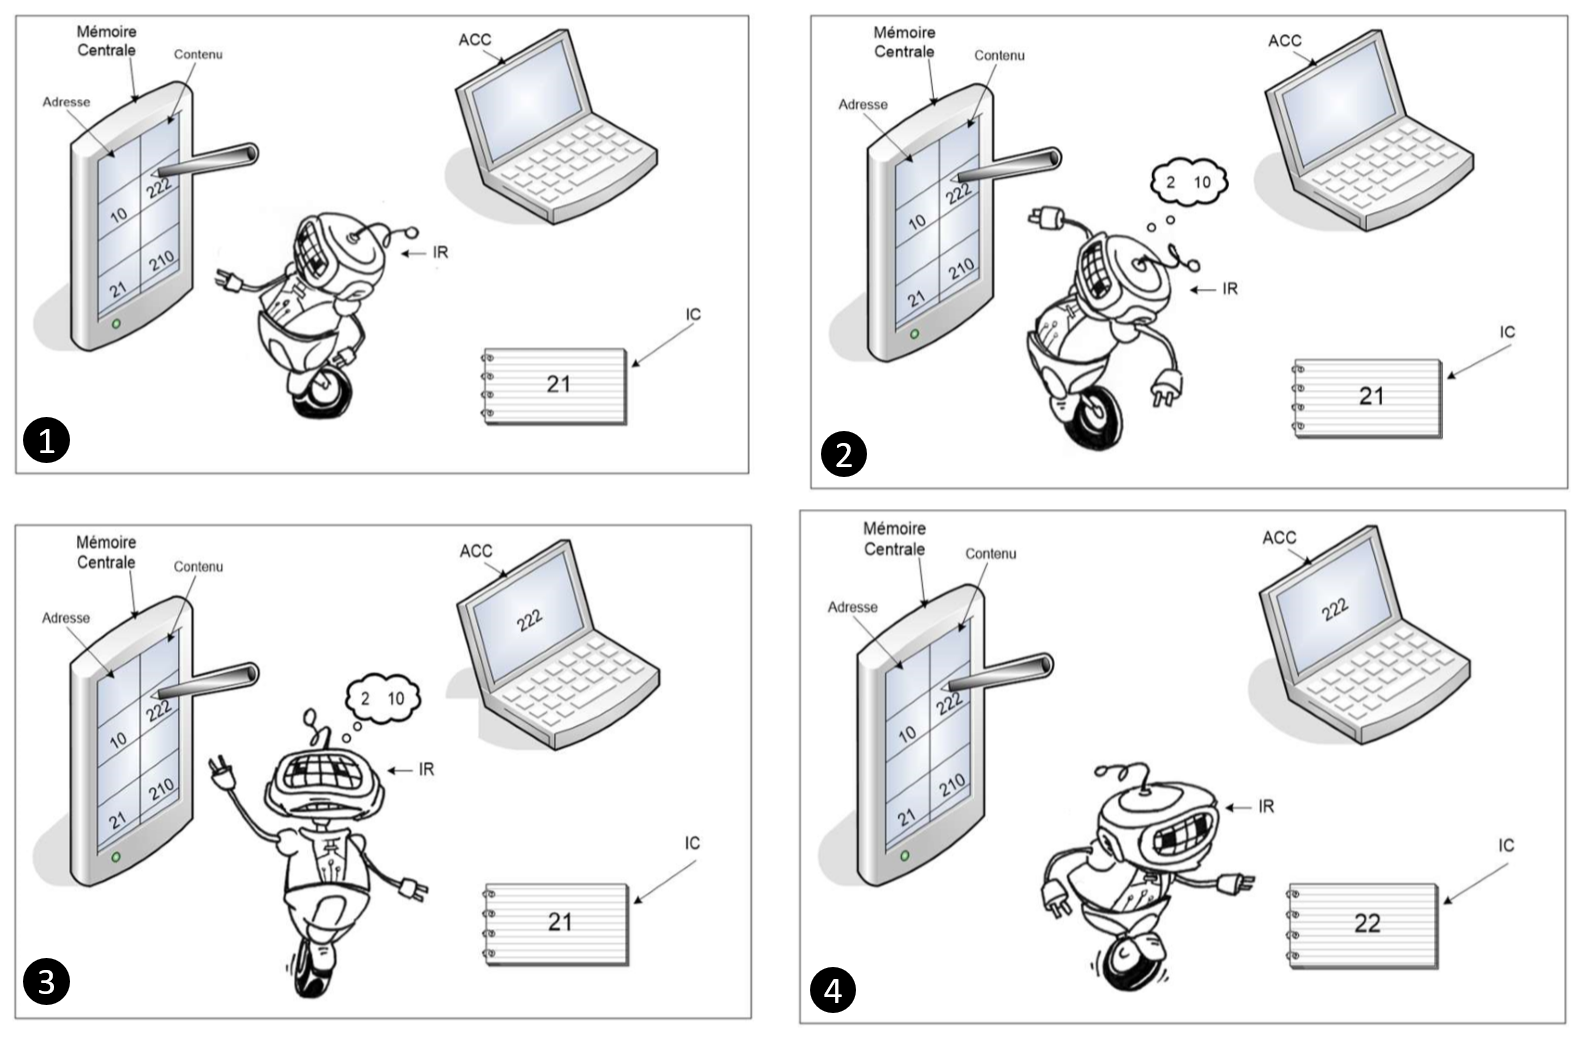
\includegraphics[width=\linewidth]{info-pho}
\caption{Fonctionnement de PHO}
\label{fig:pho}
\end{figure}
Fondamentalement, un processeur réitère ce même cycle. Il est présenté de manière un peu plus sérieuse sur la figure \ref{fig:processeurCycle}.
\begin{figure}[h!]
    \centering
    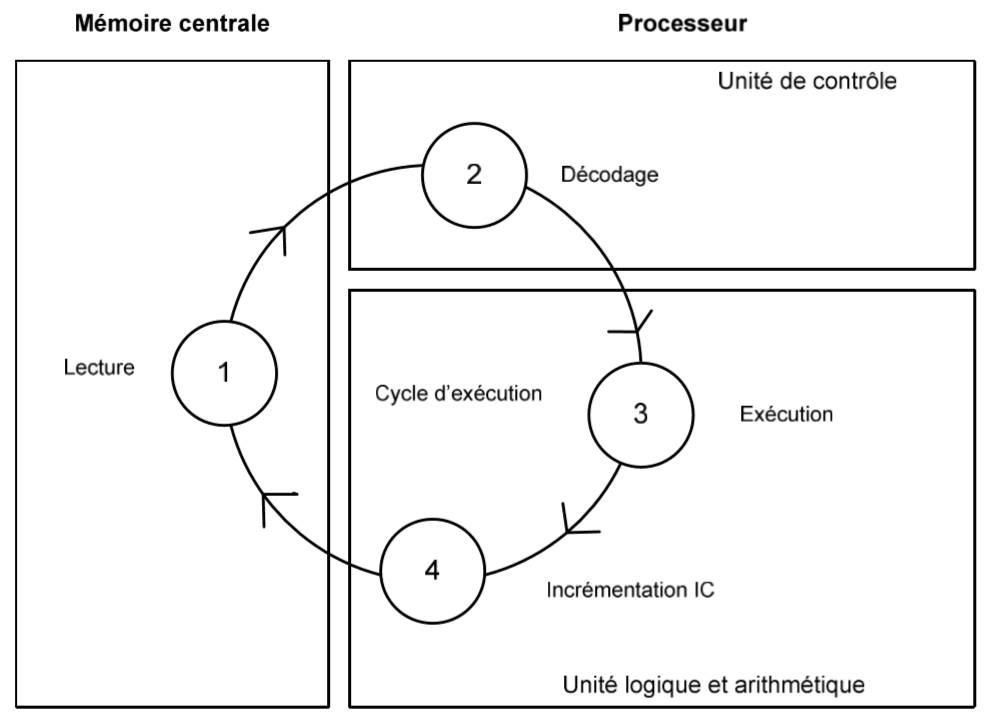
\includegraphics[width=.8\linewidth]{info-processeurCycle}
    \caption{Résumé du fonctionnement du processeur}
    \label{fig:processeurCycle}
\end{figure}
\subsection{Les instructions et leur adressage}
Dans ce qu'on vient de voir, l'instruction \underline{élémentaire} de copier une valeur dans un registre accumulateur est définie par son code, et ce sur quoi elle opère se trouve également dans le code. Les processeurs fonctionnent comme ça, encore aujourd'hui : une instruction est définie par un code, stocké en mémoire. Nous faisons la parenthèse que ce qui différencie un processeur d'un autre est son jeu d'\textbf{instructions élémentaires}. On verra ces différences par après. En tout cas, ce sont les instructions élémentaires qui définissent le processeur, son efficacité à effectuer des instructions (courtes ou longues), etc., et même si elles sont différentes, on peut les regrouper en quatre groupes :
\begin{enumerate}
\item Copie de données : entre mémoire et registre,
\item Opérations arithmétiques et logiques : calculs et comparaisons,
\item Branchements ou sauts d'instruction : interagissent sans cesse avec le CI pour passer d'une instruction à l'autre (détaillé après),
\item Entrée-sortie : lire ce CD-ROM, par exemple.
\end{enumerate}
Les instructions de branchement sont d'une importance capitale parce qu'il ne faut pas voir le fonctionnement du processeur comme une lecture tranquille d'une suite d'instructions tel un fleuve calme. Le registre compteur d'instruction se fait harceler à droite à gauche par des interruptions (cf. périphériques, chapitre \ref{chapter:peripheriques}), et certaines instructions conditionnelles requièrent non seulement interruption de l'instruction, mais redirection vers une autre instruction ! Gardons toutefois à l'esprit que ces "interruptions" ne sont que temporaires, et qu'il faut revenir à l'état initial du RI après interruption, et qu'il faut donc des instructions qui se chargent de copier les registres avant interruption : ce sont les \textbf{instructions de branchement}.
\exemple{Un \textit{if} envoie vers une toute autre instruction si la condition est validée ! Il faut revenir au cours normal des choses une fois l'instruction dans le \textit{if}.}
Nous allons à présent nous intéresser à la structure des instructions que nous avions évoquées lors du passage dédié à PH--ielz--O. En général, une instruction contient deux champs : le \textit{code instruction} et l'\textit{adresse de l'opérande}. À chaque champ est accordé une certaine longueur, par exemple respectivement 3 et 5 bits, pour une instruction de 8 bits.
$$\underbrace{010}_{\text{code}}\underbrace{01010}_{\text{adresse opérande}}  = \quad  \text{LOAD} \qquad \text{A}$$
Dans cet exemple, on a le code instruction "010" qui est l'instruction LOAD, et l'adresse opérande "01010" en binaire, soit "10" en décimal, soit "A" en hexadécimal. Il s'agit donc de charger A.
\exemple{
La copie de données : pour copier la donnée A dans la donnée B, il faut faire un LOAD A + STORE B. L'instruction "LOAD A" peut se trouver à l'adresse 21 par exemple, comme dans le cas de PHO, et "STORE B" en 22.}
\subsection{Branchements}
Les branchements sont un poil plus compliqués. Supposons le fonctionnement usuel et classique : une suite d'instructions à effectuer, et le cycle vu à la figure \ref{fig:processeurCycle} est de mise. On commence à l'instruction 1, on l'effectue, CI incrémente de 1 et on arrive à la 2, etc. Un branchement \textit{inconditionnel} rompt cette séquence et redirige vers une autre adresse. Par exemple, un branchement vers l'adresse 27, et on continue comme si de rien n'était : adresse 28, 29, ...\\
\\
Supposons maintenant un branchement \textit{conditionnel} : celui-ci, en 30 vers l'adresse 15 par exemple, renvoie, si la condition est validée, vers l'adresse 15 : un bond en arrière pour faire varier la valeur (qui valide la condition) jusqu'à ce qu'on arrive à l'adresse 30 où on re-vérifie la condition. Si celle-ci est encore validée, rebelote. En gros, voilà comment une \textbf{boucle while} fonctionne du point de vue du processeur.
\subsection{L'instruction}
\subsubsection{Code instruction}
Une instruction  élémentaire débute par un champ dit "code instruction". Il tient sur quelques bits et déclenche, après décodage, une série de sous-opérations qui aboutiront à l'exécution de telle ou telle instruction du processeur. Ces sous-opérations sont appelées "étapes atomiques" et sont coordonnées par le séquenceur, qui sera vu après.
\subsubsection{Opérandes de l'instruction}
Le code instruction est suivi d'une adresse "opérande". L'opérande indique une source ou une destination. Elle peut être une adresse en mémoire ou bien un numéro de registre dans le processeur. Naturellement, s'il y a beaucoup de choses en mémoire, l'adresse d'une donnée ou d'une instruction est plus longue. Les mémoires les plus grandes ont donc les adresses les plus longues et les instructions sont donc très gourmandes. Or il est \underline{important} de limiter la zone mémoire occupée par chaque instruction. Il faut donc \textbf{limiter la taille des adresses}. Une autre raison de limiter la taille des adresses est le \textbf{principe de localité}, qu'on décrira plus tard.
\subsection{Adressage des instructions}
Il y a tout un tas de mécanismes d'adressage des informations. Les plus intuitifs sont bien sur l'adressage \textbf{absolu}, l'adressage par \textbf{registre} (indiquer quel registre contient l'opérande), l'adressage \textbf{relatif} (déplacement "offset" par rapport à l'adresse de base. Un autre mécanisme est l'adressage \textbf{indirect} : l'adresse renvoie vers une cellule mémoire ou un registre qui contient l'adresse effective, dans le but de faciliter la manipulation d'adresses. Ce mode est utile lorsqu'un programme doit par exemple effectuer une série d'opérations sur une donnée dont on ignore encore l'adresse finale, ou si l'adresse peut varier au cours de l'exécution du programme.\\
\\
C'est l'adressage indirect, aussi appelé adressage indexé, ou adressage de registre, qui est retenu la plupart du temps. La raison principale de cela est le principe de localité, spatial et temporel :
\begin{description}[leftmargin=!, labelwidth=\widthof{\bfseries Temporelle}]
\item[Spatiale] La majorité des données et instructions accédées durant l'exécution d'un programme sont (et restent) très proches les unes des autres.
\item[Temporelle] Ce sont \textit{souvent} les mêmes opérandes qui sont utilisées dans le temps, ce qui justifie l'adressage vers une même zone de la mémoire.
\end{description}
\section{Instructions élémentaires et familles de processeurs}
Les instructions ne sont compréhensibles du processeur que de la manière dont elles sont codées. Chaque type de processeur a ses instructions codées d'une certaine manière, ce qui fait leur différence. Il y a deux grands types de processeurs : les processeurs RISC et les processeurs CISC.
\subsection{CISC : Complex Instruction Set Computer}
Pour un processeur CISC, les instructions sont de taille variable et souvent longue car on renseigne, après le code instruction, la longueur des opérandes et surtout leur adresse respective, ce qui peut être très long. Les processeurs CISC font donc beaucoup d'accès en mémoire. Leur principale qualité est leur flexibilité, leur large variété d'instructions.
\subsection{RISC : Reduced Instruction Set Computer}
Les processeurs RISC ont des longueurs d'instruction \textbf{fixes}, ce qui est leur plus grande qualité, raison pour laquelle la plupart des ordinateurs fonctionnent aujourd'hui avec un processeur RISC, avec des instructions codées sur 32 ou 64 bits pour la plupart. Ceci est donc biens moins cher en mémoire, et plus adapté à un fonctionnement en \textbf{registres}, entre lesquels il y aura beaucoup de transferts. Les programmes vont davantage s'exécuter localement par les registres et la mémoire cache (cf chapitre suivant).
\subsection{L'assembleur}
De notre point de vue, l'opération est "LOAD A" mais elle a nécessité plusieurs instructions dont le code est en binaire. Un traducteur du langage dit "assembleur" vers le binaire est un programme appelé "compilateur", comme il y en a pour les langages de programmation (= traduction du langage machine vers un langage de plus haut niveau). Une variante aux compilateurs est la présence d'\textbf{interpréteurs}, qui vont effectuer cette traduction petit à petit, plutôt que tout en un coup\footnote{Python est un langage interprété, Java est un langage compilé.}.
\section{Fonctionnement du processeur}
PH--ielz-O c'est marrant deux minutes, mais nous pouvons maintenant passer au fonctionnement \textbf{réel} du processeur. Le processeur est essentiellement un assemblage de registres et d'organes d'échange enter ces registres.
\subsection{Les registres}
Les registres sont des mémoires \underline{individuelles} de petite taille (1-8 bits) généralement très rapides, car faisant partie intégrante du processeur. Ils ont un usage spécifique, contrairement aux cellules de la mémoire centrale, que l'on verra au chapitre suivant. Les registres sont des "espaces de travail", raison pour laquelle on en trouve à peu près partout, en mémoire centrale aussi. Les communications entre registres sont assurées par le \textbf{séquenceur} dont nous parlerons après. Chaque processeur a sa panoplie de registres, tout comme la panoplie d'instructions, mais ici encore nous avons quelques registres qui constituent l'essentiel de \textbf{tout processeur}.
\bb{
\begin{description}[labelwidth=\widthof{\bfseries Compteur d'instruction (CI)}, leftmargin=!,align=right]
\item[Compteur d'instruction (CI)] Contient l'adresse de l'instruction à effectuer, et l'adresse mémoire d'où le processeur peut recopier cette instruction. Il est incrémenté en cours cours d'instruction pour pointer vers l'instruction suivante.
\item[Registre d'instruction (RI)] Contient l'instruction à exécuter. C'est ici que le décodage de l'instruction par le \textbf{séquenceur} va se faire.
\item[Accumulateur (ACC)] On ne le présente plus.
\item[Registre d'état (STAT)] Donne l'état du processeur au cours de l'instruction,  par le contenu de l'accumulateur : positif? nul? négatif? par exemple. C'est le registre qui est observé par les branchements.
\item[Registres de travail] Présents dans tous les processeurs et ce sont eux qui diffèrent d'un processeur à l'autre.
\end{description}}
La plupart de ces registres sont "programmables", ce qui veut dire que leur contenu est accessible aux programmes. En dehors du processeur se trouvent encore deux registres utiles, le registre d'adresse (\textbf{RA}) contenant l'adresse du transfert mémoire (là où écrire la donnée, ou la lire) et le registre de données (\textbf{RD}), contentant soit la donnée à écrire soit celle lue depuis la mémoire. Tout ces registres composent le cycle de fonctionnement du processeur, version \textsc{Deluxe Extended ++}, représenté sur la figure \ref{fig:processeurFinal}.

\begin{figure}[h!]
\centering
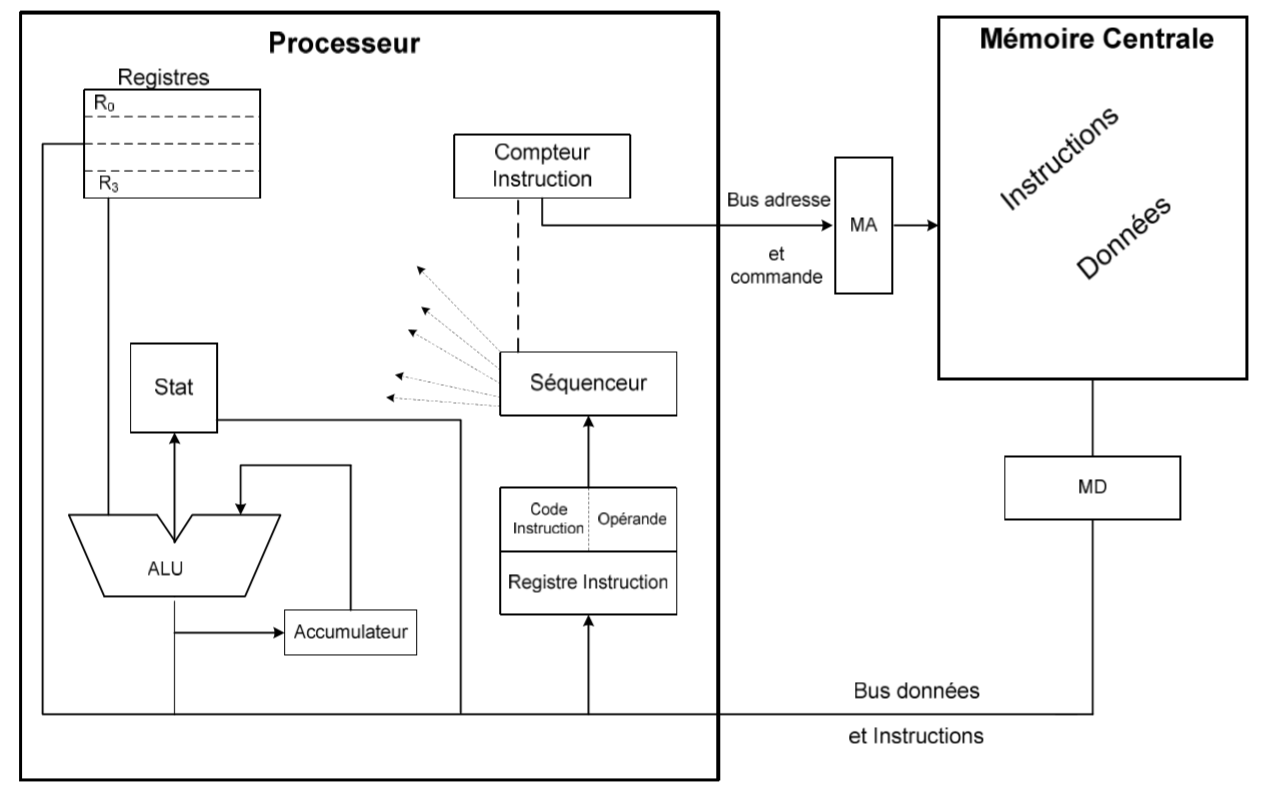
\includegraphics[width=0.7\linewidth]{info-processeurCycleFinal}
\caption{Cycle du fonctionnement du processeur}
\label{fig:processeurFinal}
\end{figure}
\subsection{Les étapes primitives, et le séquenceur}
Une instruction élémentaire telle que "LOAD A" ou "STORE B" nécessitent des étapes dites primitives, chacune de ces étapes correspondant à un cycle de fonctionnement de processeur. Le nombre de cycles effectués par seconde définit la "vitesse" du processeur : 1 GHz veut dire 1 milliard de cycles effectuées à la seconde. Nous allons voir maintenant comment chaque instruction est découpée en étapes primitives, et comment celles-ci sont coordonnées.\\
\\
La succession des étapes primitives peut se comprendre facilement avec les registres. Étudions "LOAD $R_1$, ADD $R_2$", en commençant par le "LOAD $R_1$".
\begin{enumerate}
\item Lecture : le CI place dans le RA pour obtenir l'instruction à effectuer. Celle ci est retournée dans le RD qui place l'instruction dans le RI. La phase de lecture est donc représentée par \rouge{RA $\leftarrow$ CI, RI $\leftarrow$ RD}. Elle nécessite 2 cycles.
\item Exécution : placer $R_1$ dans l'accumulateur, pour en terminer avec "LOAD $R_1$". \rouge{ACC $\leftarrow$ $R_2$}.
\end{enumerate}
Pour "ADD $R_2$", le schéma est le même, sauf qu'on a \rouge{ACC $+ R_2$} pour la phase d'exécution.

\subsubsection{Parallélisme et pipeline}
On remarque que certaines de ces étapes ont \textit{a priori indépendantes}, on pourrait techniquement déjà chercher $R_2$ en mémoire pendant qu'on place $R_1$ dans l'accumulateur ! C'est le parallélisme. 
\begin{figure}[h!]
\centering
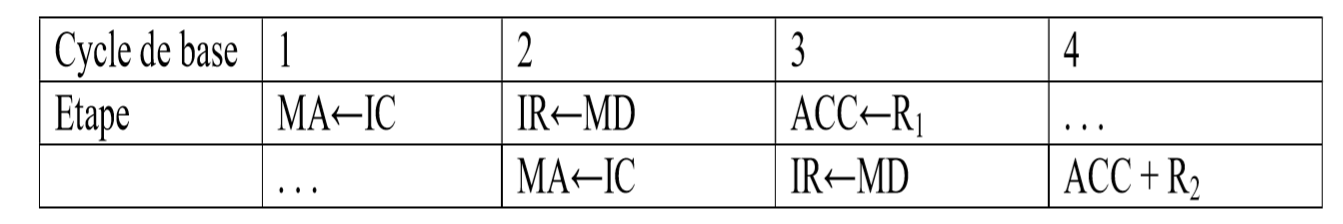
\includegraphics[width=.6\linewidth]{info-parallelisme}
\caption{Parallélisme durant l'exécution d'une instruction}
\label{fig:parallelisme}
\end{figure}
Il faut néanmoins veiller à ce que les étapes que nous voulons mener en parallèle soient indépendantes. Ceci est assuré par le \textbf{pipeline}. Comment définir le pipeline ? Très bonne question. C'est une structure fictive composée d'un chevauchement temporel mais non spatial d'instructions, selon moi. Autrement dit, l'expression "ajouter cette instruction au pipeline" se dit. À chaque instruction, le coordinateur des instructions, a.k.a le \textbf{séquenceur}, dont nous avons toujours pas parlé, analyse le contexte de l'instruction et regarde sous quelles conditions elle est admissible au pipeline. Vu l'uniformité du codage instruction des processeurs RISC, le mécanisme de pipeline est plus facile pour eux. Notons pour terminer que les instructions avec branchement sont à éviter dans le pipeline, c'est d'une évidence sans équivoque.
\begin{figure}[h!]
\centering
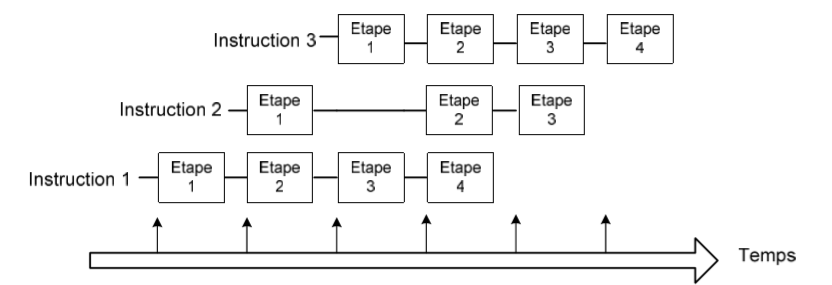
\includegraphics[width=.6\linewidth]{info-pipeline}
\caption{Pipeline}
\label{fig:pipeline}
\end{figure}
\subsubsection{Le séquenceur}
Bon, avec le nombre de fois où on a teasé ce bougre de séquenceur, est-il encore important de l'introduire ? Don't think so. C'est le chef d'orchestre du processeur. Il découpe une instruction en une séquence d'étapes élémentaires, une sorte de division spatiotemporelle.\\
\\
\wrap{}{r}{0.3}{\centering 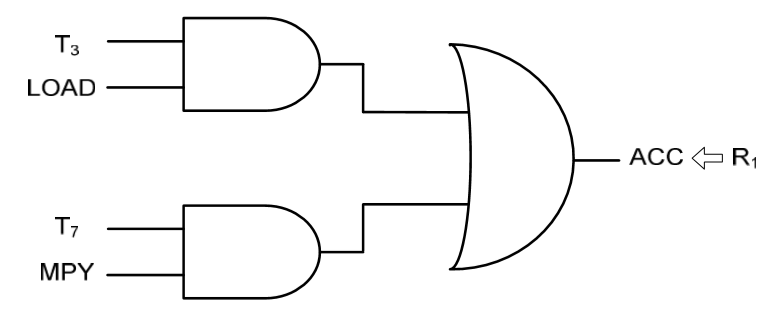
\includegraphics[width=\linewidth]{info-seqCabl} \caption{Séquenceur câblé} \label{fig:seqCabl}}
Les séquenceurs sont aussi physiques. Une manière de représenter un séquenceur est dans un circuit : un \textbf{séquenceur câblé}. Imaginons que l'étape atomique à effectuer soit ACC$\leftarrow R_1$. Ok, il faut placer $R_1$ dans l'accumulateur, mais il y a plusieurs instructions qui nécessitent cette étape atomique ! Les instructions LOAD et MPY par exemple. Le séquenceur cède la priorité à l'une d'entre elle, au choix. On se rend facilement compte sur le schéma ci-contre que pour un nombre élevé d'instructions et des variabilités au cours de celles-ci, un séquenceur câblé est un cauchemar, surtout pour les processeurs CISC, étant donné la variabilité dans la succession de leurs étapes. Une autre approche consiste en un séquenceur \textbf{microprogrammé}. Il devient un $\mu$processeur spécialisé, qui, pour chaque instruction à exécuter, va consulter une table décrivant les différentes étapes avec, pour chacune, le choix des opérations à effectuer sur les registres.
\chapter{Les mémoires}
\section{Types de mémoire}
Les mémoires sont les dispositifs permettant de stocker de l'information de manière banalisée, en quantité importante, avec aucune autre limite que \textbf{matérielle}. Les "registres" dont il avait été question dans le chapitre précédents sont trop petits et spécialisés pour être traités comme des mémoires. Les mémoires ont des caractéristiques sur base desquelles on va les hiérarchiser : entre autres mais surtout, utilisation, capacité de stockage et temps d'accès \footnote{Niveau de résolution de leur adressage, débit aussi.}. Voici sur la figure \ref{fig:hierarchieMemoires} les principaux types de mémoire dans l'ordre croissant des temps d'accès, de la taille, et dans l'ordre décroissant du coût. Une explication suivra. Gardons à l'esprit qu'une mémoire sert à deux choses : stocker et transférer de l'information (données et instructions). \\ \\

\wrap{16}{r}{0.6}{
\vspace{-1cm}
\begin{center}
\begin{tikzpicture}
\coordinate (A) at (-4,0) {};
\coordinate (B) at ( 4,0) {};
\coordinate (C) at (0,6) {};
\draw[name path=AC, very thick] (A) -- (C);
\draw[name path=BC, very thick] (B) -- (C);
\draw[name path=AB, very thick] (A) -- (B);
\foreach \y/\A in {0/Archivage,1/Mémoires de masse,2/Mémoire centrale, 3/Cache, 4/ \small Registres} {
    \draw  [dashed]($(A)!\y/6!(C)$) -- ($(B)!\y/6!(C)$)
        node[midway,above] {\A};
}
\draw [thick,->](0.3,6) -> (4.3,0) node[midway, above, rotate=-57]{ \small Temps d'accès, taille};
\draw [thick,->](-4.3,0) -> (-0.3,6) node[midway, above, rotate=57]{\small  Coût};
\end{tikzpicture}
\end{center}
\caption{Hiérarchie des niveaux de mémoires}
\label{fig:hierarchieMemoires}
}
\textit{Commençons} par distinguer les mémoires par leur \underline{légèreté}. Certaines mémoires sont utilisées en se remplissant et se vidant durant leur utilisation : ce sont les mémoires \textbf{vives} (\textbf{mémoire RAM}), qui alimentent le processeur en instruction. Rappelons que les mémoires ne stockent rien que des bits, qui peuvent être données ou informations, la mémoire ne le sait pas, elle stock des bites et c'est tout, la coquine. D'autres mémoires sont \q{permanentes} dont on conserve le contenu entre deux utilisations des programmes ou de la machine. Ce sont les \textbf{mémoires ROM}.  \\ \\ 
\textit{Ensuite}, définissons le temps d'accès. Il y a plusieurs phases pour accéder complètement à une mémoire. La succession de ces phase constitue le temps d'accès.
\begin{enumerate}[label = \roman*.]
\item Phase de préparation : durée qui dépend d'un accès précédent et de la position dans laquelle cet accès a laissé la mémoire,
\item Phase de transfert, qui dépend du volume de données à transférer et des performances de la mémoire.
\end{enumerate}
C'est surtout sur base du temps d'accès qu'on va hiérarchiser les mémoires.

\section{Hiérarchie des mémoires}
Les mémoires les plus rapides mais aux capacités les plus limitées sont les \textbf{registres} : nombre limité d'octets, et le temps de réponse détermine la vitesse du processeur (cf. étapes atomiques). Elles sont suivies par les mémoire "cache", et ainsi de suite suivant la figure \ref{fig:hierarchieMemoires}.

\subsection{Mémoire cache et mémoire centrale}
La mémoire centrale est aussi appelée RAM, pour \textit{Random Access Memory} parce que l'accès à cette-dernière se fait de la même manière et prend le même temps. Il s'agit d'un mode d'accès dit "direct" : la mémoire centrale permet d'adresser des cellules de la taille de l'octet ! Mais en pratique, c'est un plus grand nombre d'informations qui est véhiculé, pour les raisons qui suivent. \\ \\
Si on veut runner un programme dans lequel sont souvent utilisées les mêmes instructions, on pourrait techniquement les stocker dans une mémoire plus petite pour qu'elle soit plus rapide qu'une mémoire plus grosse comme la mémoire RAM. C'est la raison pour laquelle un processeur se verra souvent adjoint une mémoire à capacité plus réduite, et par conséquent \textbf{beaucoup plus rapide : la mémoire cache}.  Les mémoires cache et RAM ne fonctionnent pas quand elles ne sont pas alimentées en courant. La mémoire centrale, la mémoire cache, et les registres sont des mémoires volatiles. Résumons enfin le rôle de la mémoire centrale :

\bb{\begin{center}
Le rôle de la mémoire centrale est de contenir toutes les données et instructions nécessaires pour l'exécution des programmes par le processeur, ainsi que d'assurer les échanges avec les unités périphériques.
\end{center}}

\subsection{Mémoires secondaires/de masse}
\begin{itemize}
\item Non-volatiles
\item Données écrites sous forme de champ magnétique
\item En dehors de l'unité centrale
\item Contenu accessible à tout moment, contrairement à la RAM qui nécessite une alimentation.
\item Les cellules adressables sont atteintes en mode "direct" : \textbf{mode d'accès "aléatoire"}, mais pas comme la RAM parce que là, le temps d'accès dépend de la position courante de la tête de lecture et du temps requis pour que celle-ci se déplace jusqu'à l'endroit voulu.
\item Le temps d'accès dépend de la position de la tête de lecture et du déplacement de cette-dernière.
\item[$\Rightarrow$] Accès lent (parce que loin et grand), permanent, direct.
\end{itemize}

Comme on parle de mémoire, on parle surtout de transfert de mémoire. De la mémoire centrale au processeur on transférait quelques blocs. Des mémoires secondaires à la mémoire centrale on transfère un nombre beaucoup plus grand comme 4096 octets. Tout doit transiter par la mémoire centrale. Les mémoires secondaires contiennent \textbf{tous les programmes}, y compris le système d'exploitation (des dizaines de millions de lignes de code pour Linux). Le fait que l'accès en mémoire secondaire soit permanent et direct est utile pour en construire des extensions de mémoire (\textit{disques durs externes}).
\subsection{Mémoires d'archivage}
C'est une manière de stocker des copies de données dont l'accès immédiat n'est pas nécessairement requis. Elles sont donc souvent constituées de supports amovibles. Les mémoires d'archivage servent plus généralement à libérer de l'espace sur les mémoires de masse (disque dur) en effectuant une copie de leurs données de manière à ce qu'une reconstitution soit possible. Finalement, comme elles sont utilisées pour la \textbf{copie de données}, elles sont du type à accès \textbf{séquentiel}.

\section{Transferts de niveau}
La hiérarchie des mémoires a permis de distinguer les différents types de mémoire selon leur utilisation, vitesse, capacité de stockage, et place dans la communication avec le processeur. On va voir maintenant comment les transferts se réalisent entre les différents niveaux de mémoire.  \\
\\
Le processeur a besoin d'information, et il s'en fout d'où elle provient : elle doit juste arriver rapidement. Il s'adresse donc à la mémoire la plus rapide : la mémoire cache. Si ce qu'il cherche n'est pas dedans, il va chercher dans la mémoire centrale, et si elle n'est pas là il va chercher dans le disque dur. Mais si il doit effectuer un tour dans une mémoire plus loin (centrale, secondaire) il rapatriera un \textbf{bloc} pour éviter de devoir y retourner. Les concepteurs d'ordinateur doivent donc \textbf{définir} cette unité d'échange, le \textbf{bloc}, avec les meilleures performances malgré les contraintes matérielle et économique. L'adressage est alors par bloc ce qui permet facilement de voir si une donnée est dans la mémoire cache ou non. Si le bloc y est, alors oui. Si une adresse est écrite en Hexadécimal, les 12 chiffres de droite seront réservés à la localisation dans le bloc : un bloc a donc une taille de 4096 octets dans ce cas. \\ \\
Comme la mémoire cache a une capacité de stockage assez réduite, son contenu est sans cesse écrasé, mais comme il s'agit d'une copie tout va bien. Si en revanche la donnée est changée au cours du programme, alors il faut la rapatrier au sein de la mémoire lente (pour être stockée).
\subsection{Fonctionnement de la mémoire centrale}
\subsubsection{Mémorisation : DRAM ou SRAM}
\begin{wraptable}[7]{r}{0.4\textwidth}
\vspace{-0.5cm}
\centering
\begin{tabular}{|l|cc |}
\hline 
 & DRAM & SRAM \\
 \hline
Prix & - & + \\
Capacité & + & - \\
Rapidité & - & + \\
Nature & Capacités & Bistables \\
Volatile & Oui & Oui \\
\hline
\end{tabular}
\end{wraptable}
Les mémoires centrales sont construites sur la base d'une technologie de type DRAM, pour \textit{Dynamic RAM}. Ces mémoires sont de types \q{dynamique}, nécessitant rafraîchissement, contrairement aux SRAM qui valent pour \textit{Static RAM}. Les DRAM consistent en un circuit de capacités tandis que les SRAM ont une technologie proche des processeurs. On les construit donc avec. Les mémoires centrales sont donc des DRAM et les mémoires caches sont des SRAM, beaucoup plus rapides mais plus chères.
\subsubsection{Adressage et transferts : registres}
\begin{itemize}
\item[RA] Le Registre d'Adresse contient l'adresse de l'octet à lire ou à écrire. Si le RA est de 32 bits, il couvre un espace adressable de $2^{32}$ octets. Le décodeur d'adresse reçoit en entrée le RA et doit sélectionner l'octet voulu selon ce qu'il y a dans le RA. Dans le cas d'un RA de 32 bits le décodeur devient hyper complexe et il faut donc une nouvelle manière d'adresser : \textbf{l'adressage bidimensionnel}.
\item[RD] Le Registre des Données contient les données à lire ou à écrire en mémoire centrale. La taille du RD conditionne la taille de l'information que l'on récupère lors d'un accès en mémoire centrale. Elle est typiquement de 8 octets.
\end{itemize}

\subsection{Mémoire virtuelle}
il se fait quand même tard (5h00, c'est le confinement tqt). Bref, le concept de "mémoire virtuelle" vient de l'intention de berner les programmes. Ceux-ci se verraient mieux vivre dans l'illusion qu'ils ont toute la mémoire à eux et rien qu'à eux alors que mdr ils sont full à tourner dessus. La mémoire virtuelle se trouve au sein de la mémoire centrale. Elle est en effet utile parce que:
\begin{itemize}
\item Les programmes peuvent prendre plus de mémoire que ce que la mémoire centrale peut offrir,
\item Les programmes sont codés pour gérer plusieurs situations mais qui ne se déroulent pas simultanément. Donc ils prennent bcp de place théoriquement alors que si on les laisse occuper la mémoire voulue en temps voulu il n'y a pas de problème. Les mettre sur une mémoire virtuelle est donc une bonne idée.
\item Multitâche : la simultanéité n'est possible qu'en partageant à tour de rôle le processeur.
\item Variations de l'espace mémoire disponible : l'espace réellement occupé en mémoire centrale en continu !
\end{itemize} 

Oh \textsc{Putain} j'ai dormi je suis en pleine forme (il est 17h00). Il faut tout ré-expliquer ! Les programmes sont des suites d'instructions et il se peut qu'ils doivent occuper une quantité de stockage que la mémoire centrale ne puisse pas stocker. Comment faire ? De plus, il se peut qu'un même programme fonctionne plusieurs fois, et que plusieurs programmes fonctionnent simultanément. En gros on se rend compte qu'il y a un problème pour le fonctionnement d'un programme parce qu'entièrement il est énorme mais il utilise en 1 seul instant beaucoup moins que ce qu'il prévoit ! Alors l'idée est de le \underline{berner} en lui donnant l'illusion qu'il a accès à toute la mémoire qu'il veut. La manière de procéder est la suivante :
\begin{description}[leftmargin = !, labelwidth=\widthof{\bfseries Pagination }]
\item[Pagination] Un \textbf{programme} est découpé en un ensemble de segments de même longueur, des \textbf{pages}. De son point de vue, il voit qu'il est coupé en pages de manière continue. 
\item[$\Rightarrow$] Une page contenant un certain nombre d'instructions (typiquement 4096 octets), elle est active dans la mémoire centrale quand elle est utilisée uniquement.  
\end{description}
Ceci permet de mieux gérer l'espace disponible étant donné que l'espace occupé par les programmes est très variable.
\subsection{Pagination} \label{subsection:pagination}
La gestion de mémoire doit passer par une différenciation entre l'adresse "logique" qui est celle vue par le programme (cf. mémoire virtuelle) et les adresses réelles des cellules de ce programme qui sont placées en mémoire centrale. Cette différenciation est garantie par la \textbf{pagination} avec le concept de table des pages. \\ \\
En effet, le programme est découpé en pages, et chaque page occupe un espace réel dans la mémoire centrale lorsqu'utilisée. Comme toutes les pages du programme ne sont pas dans la mémoire centrale en même temps, il serait judicieux pour le processeur de savoir si l'instruction à lancer (qui est contenue dans une des pages du programme) 
\wrap{20}{r}{0.65}{
\centering
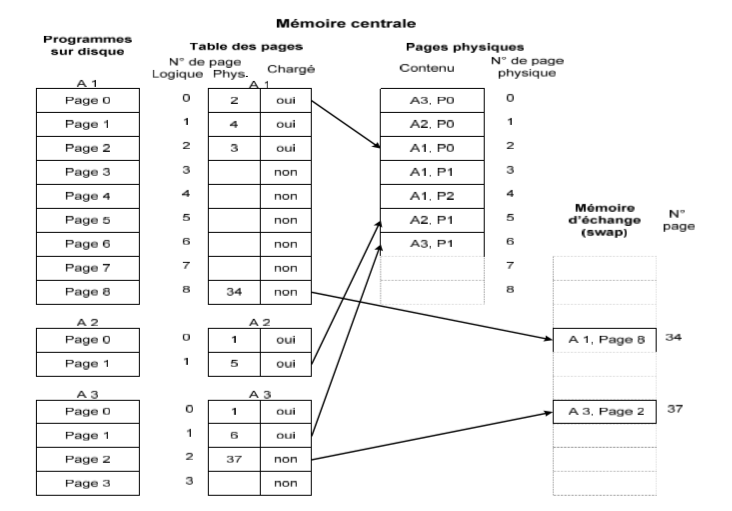
\includegraphics[width = 0.65\textwidth]{info-tablePages}
\caption{Fonctionnement de la mémoire centrale à travers la mémoire virtuelle.}
\label{fig:memoireCentrale}
}
est dans la mémoire centrale ou non, pour savoir s'il faut la chercher dans la mémoire secondaire ou non. Ceci se fait via une table des pages, qui est créée par le système d'exploitation, et à chaque programme fait correspondre le numéro de page logique au numéro de la page physique si la page est dans la mémoire centrale. \\
\\
Ainsi, pour qu'un programme puisse accéder à un octet, il ne suffit que de transposer le numéro de page logique en numéro de page physique : l'octet a la même adresse relative (\textit{offset}) dans la page, qu'elle soit virtuelle ou réelle. Si cette page physique se trouve dans la mémoire centrale, alors c'est gagné, sinon il faut aller la chercher sur le disque dur et la copier dans la mémoire centrale : on voit que la mémoire secondaire joue un rôle d'extension de mémoire. \\
\\
Reste à savoir quelle donnée remplacer lors d'un transfert de la mémoire secondaire $\longrightarrow$ mémoire centrale. La table des pages est donc complétée d'informations complémentaires pouvant faire la hiérarchie des éléments à supprimer : moment d'installation, du dernier accès, nombre d'accès, et pour savoir s'il faut rapatrier la page vers la mémoire secondaire, il faudrait également avoir une information sur si oui ou non la page a été altérée pendant le fonctionnement du programme. Tout ceci résume le rôle de la table des pages.

\bb{Table des pages :
\begin{itemize}
\item Pagination : permet de faire la distinction entre les pages logiques (programme) et les pages physiques (réelles, mémoire centrale).
\item Accès mémoire : à la simple lecture du numéro de page, le processeur sait s'il doit chercher ou non l'information dans la mémoire secondaire.
\item Ne sont en mémoire centrale que les pages nécessaires à l'instruction actuelle des programmes : économie de l'espace géré, car les programmes occupent un espace très variable.
\end{itemize}}

\subsection{Unité de gestion de mémoire : MMU}
Le registre d'adresses RA ne se charge donc plus d'une adresse complète telle que présentée par le programme (instruction XXXXXX) mais d'une composition d'un numéro de page physique (trouvé dans la table des pages) et d'une adresse relative à la page. Cette composition est réalisée par un organe accolé à la mémoire centrale appelé \textit{Memory Management Unit}, MMU.
\subsection{Mémoire associative : TLB}
Comme l'accès en mémoire centrale est déjà quelque chose de lent, il faut une annexe à la table des pages qui soit ultrarapide : c'est la TLB, une mémoire de très petite capacité ultrarapide (fait partie de la mémoire cache) qui contient une copie des données les plus souvent utilisées dans la table des pages, avec quelques informations en plus comme cette-dernière. \\
\\
Le TLB se devant d'être ultrarapide, c'est une mémoire à laquelle on va accéder non par adresse mais par contenu. C'est plus rapide parce qu'on ne parcourt pas tout l'espace mémoire mais on recherche un contenu précis. On ne fournit pas une adresse, juste le numéro de la page précis. Pour illustrer, c'est comme si on avait deux situations : la première on vous donne un nom et on vous demande de retrouver qui c'est... ça mettra du temps parce que vous devez fouiller toutes les têtes dans votre mémoire. La deuxième situation : on vous donne un visage et c'est tout de suite plus facile à reconnaître ! Dans le cas du TLB, on parle en numéro de page logique. Si le numéro a été trouvé, alors le numéro de page physique est généré automatiquement par l'unité de gestion de mémoire (celle qui gère la juxtaposition des pages physiques dans la mémoire centrale).

\section{Antémémoires, mémoires caches}
Comme déjà mentionné, l'antémémoire/mémoire cache est une mémoire très petite très rapide (car réalisée en SRAM) adossée au processeur. Elle contient une copie des instructions les plus fréquemment ou récemment utilisées. Lorsqu'un accès en mémoire est nécessaire, c'est tout un bloc qui est rapatrié en mémoire cache (blocs de 4 à 64 octets), parce qu'il est probable que l'instruction suivant est proche de l'instruction actuelle (principe de localité spatiale et temporelle).
\subsection*{Lignes de cache et accès à la mémoire cache}
La mémoire cache est constituée de blocs comme on l'a vu, mais qu'on va appeler "lignes" à partir de maintenant, qui sont au nombre, par exemple, de 256 et constituées chacune de 16 octets. 256 lignes de 16 octets nous fait un nombre de 4096 octets pour la mémoire cache. La mémoire centrale est elle, bien sûr, beaucoup plus grande. Si l'on veut transférer 16 octets, soit une ligne, vers la mémoire cache il faut s'assurer que l'emplacement soit libre ! Et même plus précisément, un ensemble de 16 octets est adressé en mémoire centrale par un code hexadécimal. Et la manière dont l'adresse sera lue est la suivante : \bleu{à droite c'est l'adresse relative dans la ligne}, \green{au milieu c'est le numéro de la ligne}, et \rouge{à gauche c'est le \textit{tag}, l'adresse qui lui fait tenir compte d'où il vient dans la mémoire centrale}. Prenons les exemples de l'octet 4480, 4496, et puis 8592 : 
\begin{eqnarray*}
4480 &=& 1\times 16^3 + 1\times 16^2 + 8\times 16^1 + 0\times 16^0 \\
&\Rightarrow& \underbrace{\boxed{\rouge{1}}}_{\text{tag}}\qquad \underbrace{\boxed{\green{18}}}_{\text{ligne}}  \qquad \underbrace{\boxed{\bleu{0}}}_{\text{octet}} = 1180 \\
4496 &=&  \boxed{1} \qquad \boxed{19} \qquad \boxed{0}  \qquad \ \ = 1190 \\
8592 &=&  \boxed{2} \qquad \boxed{19} \qquad \boxed{0} \qquad \ \ = 2190
\end{eqnarray*}

Pour les deux derniers, on voit qu'il y a un conflit parce qu'ils occupent la même ligne de la mémoire cache. Ces conflits ont réglés par la \textit{tag table} qui indique le tag qui correspond à chaque ligne. Donc en résumé, lorsque le processeur cherche une instruction, il regarde d'abord dans le TLB pour voir si la page logique s'y trouve. Si elle s'y trouve en effet, il doit vérifier que l'octet se trouve bien en cache et cela se fait en examinant la \textit{tag table}, qui est là pour associer chaque ligne de cache à une localisation en mémoire centrale. Si l'octet est bien en cache (que la ligne de bon tag y est) alors il est envoyé au processeur.

\begin{figure}[h!]
\centering
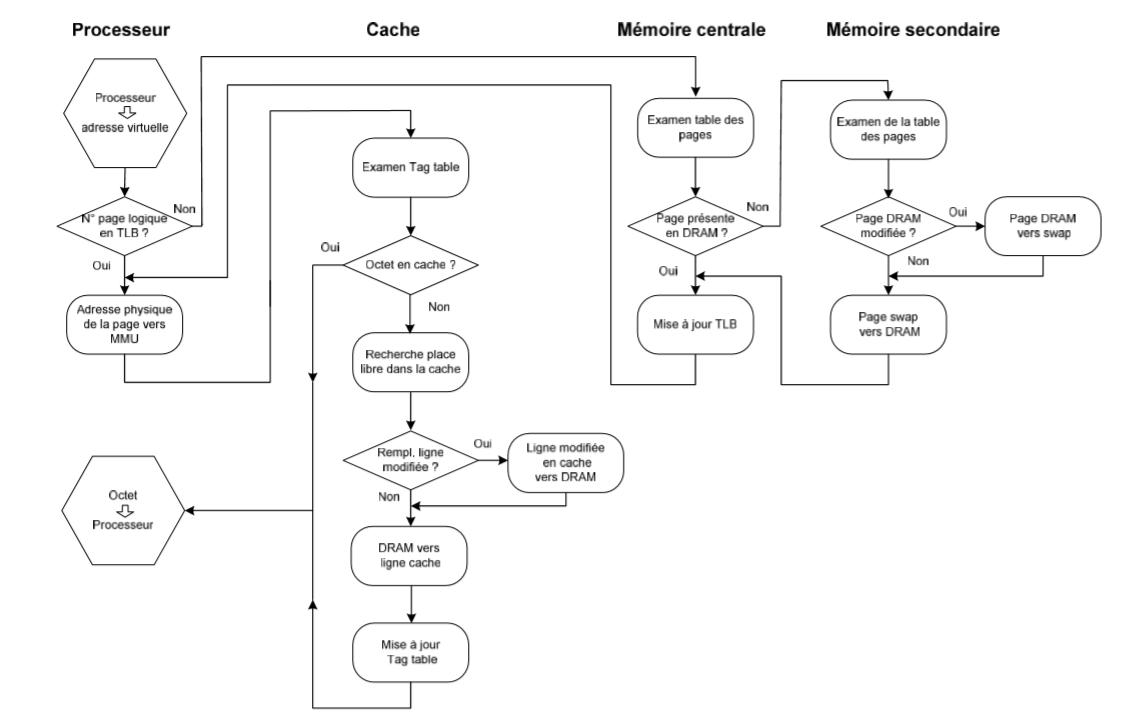
\includegraphics[scale=0.5]{info-memoireResume}
\caption{Résumé de l'accès à la mémoire, niveau par niveau.}
\label{fig:memoireResume}
\end{figure}
\chapter{Entrées/Sorties et périphériques}\label{chapter:peripheriques}
\section{Généralités}
On va parler dans ce chapitre des manières d'entrer de l'information dans l'ordinateur et de faire sortir des informations de l'ordinateur via des mécanismes IO \textit{Input/Output}. Sans accès au CPU (processeur) l'ordinateur est complètement utile, et la communication avec lui se fait à travers les \textbf{périphériques}, comme les claviers/souris, la commande vocale, gestuelle ... Mais ce chapitre parlera d'un mécanisme tout à fait général comme le \textbf{mécanisme d'interruption}.\\
\\
Rappelons-nous que le processeur n'accepte que des bits, des 1 ou des 0. Les différents périphériques envoient de l'information avec un débit qui leur est propre et cette information doit être traduite en 1 et 0. L'idéal est que cette traduction en bit se fasse directement du côté des périphériques parce que le processeur fonctionnerait mieux s'il s'en foutait de l'origine de l'information. \\
\\
Chaque périphérique est donc défini par un mode d'interaction, un \textbf{pilote}, qui n'est rien d'autre qu'un programme, qu'il va falloir installer. Par exemple, "save file" est traduit en bits par un pilote. Donc pour communiquer avec les périphériques, \textbf{le processeur a besoin d'un pilote}. Du côté du périphérique, il y a un \textbf{contrôleur}. La communication entre le processeur et le périphérique se fait donc en réalité entre le pilote et le contrôleur. 

\exemple{
Dans l'ordre croissant du débit d'information : clavier, souris, voix, scanner, imprimante, disque dur.
}

En général, les pilotes sont déjà installés dans le système d'exploitation, mais ils peuvent quand même être installés.
\section{Appareils périphériques (éléments de culture générale)}
\subsection{Sauver de l'information : disque dur}
\subsubsection{Disque magnétique}
Quand on achète un disque dur externe, il est souvent magnétique. C'est un périphérique consistant en une extension du disque dur. \\
\\
Fonctionnement : bras de lecture séparé de la bande magnétique de quelques microns, vitesse de lecture d'environ 10000 tours/mins. Si le disque dur est défaillant il est très fort probablement perdu à jamais. De même, quand on débranche brusquement un disque dur magnétique, possible que la tête de lecture ne revienne pas à sa position de repos et "blesse" la piste magnétique. \\
\\
Ici, la vitesse de lecture est la même mais c'est la densité d'information dans les bandes qui s'adapte.
\subsubsection{Disque optique}
Grosse différence : c'est la vitesse de lecture qui s'adapte, et la densité d'information qui reste la même.

\subsection{Écrire de l'information : le clavier}
Quand on appuie, le signal est envoyé au contrôleur du clavier, et le signal est traduit en ASCII et envoyé au CPU (attention aux utilisations de plusieurs touches). Le pilote peut modifier la lecture du clavier !
\subsection{Lecture d'information : les écrans}
\subsubsection{Écran cathodique}
Les canons à électrons envoyaient les couleurs élémentaires RGB, et il fallait coder à l'avance la trajectoire et l'intensité des électrons (accélération). On obtenait alors  un mélange des 3 couleurs.
\subsubsection{Moniteurs}
Il y a deux éléments importants : la résolution et la fréquence de rafraîchissement.

\section{Raccordement des périphériques}
Le mode de raccordement le plus répandu aujourd'hui est l'USB, qui est un bus (mélange contrôleur -- fil). Les raccords USB sont des raccords assez lents.

\section{Mécanisme des interruptions}
\exemple{Qu'est-ce qu'il se passe lors d'un KeyListener de Java ? \\
\\
Quand on appuie sur le clavier, on déclenche une interruption. Chaque interruption déclenche un programme qui va lire la touche qui a provoqué l'interruption et envoyer l'information au CPU en disant "je t'interromps et voilà l'information que tu es censé recevoir". Le CPU lit l'information et la \textbf{gère}. Exemples :
\begin{itemize}
\item Le \textsc{ctrl+alt+delete} lance le gestionnaire de tâches.
\item \textsc{ctrl + s} lance le programme de sauvegarde
\item ...
\end{itemize}
Dans le cas d'un KeyListener, tout part encore d'une interruption mais l'évènement est codé et arrive jusqu'à notre programme. De même, quand une imprimante n'a plus d'encre, et elle envoie une interruption qui va, lorsque lue par PHO, afficher une fenêtre.
}
Le périphérique s'identifie au CPU par ses lignes d'interruption. Tout le contexte d'exécution du programme interrompu doit être sauvegardé pour être repris par après : tout ce qui est dans le registre, dans le carnet d'instruction doit être sauvegardé dans une pile, et puis tout devra être remis après l'interruption.

\bb{\begin{center}
L'interruption d'un programme ne va pas sans la restitution exacte du contexte d'interruption du programme.
\end{center}}
L'interruption est une modification du cours normal des instructions et se traduit en fait par un branchement vers une adresse où débute le traitement de l'interruption, qu'on appelle ISR pour \textit{Interrupt Service Routine}. Voilà comment fonctionne le mécanisme d'interruption, ou l'instruction de l'ISR :
\begin{enumerate}
\item Sauvegarde du registre compteur d'instruction (CI), registre où subsiste le temps d'une instruction l'adresse de l'instruction que le programme interrompu s'apprêtait à effectuer.
\item Sauvegarde des autres registres du processeur avec le contenu que le programme interrompu y avait laissé. Ce contenu est stocké dans une portion de la mémoire centrale sous forme de pile (\textit{stack}).
\item Une fois ces précautions prises, l'ISR s'occupe de l'évènement qui a causé l'interruption.
\item La cause de l'interruption étant traitée, l'ISR recharge les registres du processeur qui s'y trouvaient au moment de l'interruption et termine par le registre CI. Le programme interrompu est ainsi entièrement rétabli.
\end{enumerate}


Plus concrètement, un périphérique annonce par une interruption un \textbf{changement d'état} qui doit être géré par le programme d'interruption (s'assure du transfert de la donnée). De plus, un ordinateur est connecté à plusieurs périphériques simultanément, donc il se peut que des interruptions se chevauchent, ce qui doit être géré. Les périphériques envoient alors des \textit{demandes d'interruptions} ou \textit{Interrupt Request} (IRQ) au processeur via le contrôleur. Chaque contrôleur de périphérique reçoit donc un numéro d'IRQ, ce qui se traduit en réel par un canal par lequel véhiculer l'interruption jusqu'au processeur. L'IRQ ne sera prise en compte que lorsque l'ISR traitant l'interruption précédente le permettra. Typiquement lorsqu'elle aura fini de copier l'état du CI et des autres registres du CPU. \\
\\
Par ailleurs, des interruptions peuvent être générées par le processeur lui-même, elles ne sont pas propre aux périphériques : une erreur de programmation comme la division par 0 peut lancer des interruptions, un programme qui effectue un appel de fonction aussi, un programme qui se plante, par exemple. La simple \textbf{horloge} aussi peut déclencher une interruption. Pourquoi ? Parce qu'en fait quand il y a plusieurs programmes qui fonctionnent en même temps, chacun doit avoir la main au processeur, mais pas les deux en même temps. Chacun aura la main séparément, dans un semblant de simultanéité (trop vite pour qu'on se remarque). \\
\\
Prenons comme exemple le transfert de fichiers vers un périphérique de type disque dur. Le pilote du processeur demande au contrôleur du périphérique de se préparer à recevoir une telle quantité de données. \q{réserve moi ...MB de place}. Une fois que le message est passé, le CPU reprend son cours de rôle et les Bytes transitent de la mémoire centrale vers les périphériques. On notera que tous les périphériques doivent avoir un accès privilégié à la mémoire centrale.

\chapter{Les logiciels --- le système d'exploitation}
\section{Introduction --- le secret vs l'Open Source}
C'est un programme, écrit dans un langage de programmation (écrit en C pour la plupart, Java pour certains). C'est lui qui va chercher les pages qu'il manque dans la mémoire, lui attribue un canal de communication pour les périphériques, lui qui gère le partage entre les interruptions, le partage entre les utilisateurs, etc... En gros c'est le programme central et de fait le premier qui se lance quand la machine est démarrée. \\
\\
Le système d'exploitation gère les ressources pour nous. On considère par exemple que les pilotes des périphériques sont contenus dans l'OS. Il faut pouvoir utiliser le système d'exploitation par un programme aussi. Il a donc deux interlocuteurs : nous, et tous les programmes, car ceux-ci interagissent également avec via "save file", etc.\\
\\
Il y a  beaucoup beaucoup de systèmes d'exploitation, qui se font tous la compétition parce que c'est \textsc{le} programme qui régit le fonctionnement de l'ordinateur. Par exemple, on installe Windows mais on est très souvent amené à utiliser Office aussi, et l'argent revient à la même personne qui a orienté Windows vers le téléchargement de Office : BILL GATES. Par conséquent, c'est très difficile de manipuler un système d'exploitation parce que le code source très souvent masqué, le programme n'étant disponible que sous sa version exécutable avec des 1 et des 0.\\
\\
Vint alors monsieur \textsc{Linus} qui mise sur la collaboration. Il écrit un système d'exploitation et partage le code et ouvre la porte à la modification du code et surtout à \textbf{l'amélioration}, ce sont les prémices de l'Open Source.

\section{Généralités}
L'OS est un interface entre le matériel de l'ordinateur (GPU, CPU, ...) et les utilisateurs (nous via les périphériques, les programmes, etc.). Il gère donc le matériel à travers les utilisateurs : il gère la mémoire, les process, les fichiers, et les réseaux.
\subsection{Rôles de l'OS}
Il gère :
\begin{itemize}
\item Traitement des fichiers,
\item Traitement et gestion des entrées sorties,
\item Teste la mémoire, teste le processeur, teste l'accès au disque dur, et une fois cela fait, un  petit morceau de l'OS va chercher le restant de l'OS dans le disque dur et le met dans la mémoire RAM pour pouvoir démarrer.
\end{itemize}
Il y a eu une évolution historique des systèmes d'exploitation : d'un ordinateur avec une tâche unique, puis un seul utilisateur  avec tâches multiples, puis plusieurs utilisateurs en multitâche, jusqu'au fonctionnement de plusieurs ordinateurs.\\
\\
L'OS est un programme "event-driven" c'est à dire qu'il intervient que quand on lui demande d'intervenir, via un programme ou une commande. Il prend le contrôle en réponse à une requête de l'utilisateur ou par le jeu des interruptions.
\section{Organisation en processus} \label{section:processus}
Un process/processus est un programme en exécution. Avant d'être exécuter il est dans la mémoire, prêt à être exécuté. Quand on clique dessus pour le lancer, son chargement en mémoire centrale le transforme en processus. Quand on le lance, il va être mis dans une liste de processus prêts à l'emploi et c'est le système d'exploitation qui va décider de quel processus peut s'exécuter. \\
\\
Un processus s'exécute et il peut se passer diverses choses : l'OS peut décider de donner la main à un autre processus, ou il peut être interrompu par manque de ressources etc. Mais la plupart de temps, l'OS va \textbf{donner la main aux différents alternativement} : il donne la main au processus 1, puis 2, puis 3 etc. en allouant un certain temps à chacun, si ceux-ci ne se bloquent pas eux-mêmes. Une fois tous les processus ayant eu la main, l'OS refait un tour, et ainsi de suite, donnant un \underline{semblant de simultanéité} : on n'a pas autant de processeurs que de processus. On peut s'en convaincre en observant dans le gestionnaire de tâches qu'il y a énormément de processus en même temps.
\subsection{Le bloc descripteur de processus}
On sait que le processus est un programme en exécution. On distingue deux modes de processus : les \textbf{processus utilisateur} et les \textbf{processus système}. Les processus système sont intégrés dans l'OS et sont autorisés à exécuter certains types d'instructions et accéder à certaines zones de la mémoire centrale ou autres registres. Ainsi, lors de l'exécution d'une procédure entrée-sortie par exemple, un processus en mode utilisateur sera restreint par ses limites d'accès et se verra obligé de passer la main à un processus en mode système, et c'est l'OS qui gère ce "passage de main" parce que c'est le seul qui peut changer quelque chose dans le registre d'état. Ainsi, afin de gérer les différents processus, l'OS doit en connaître, entre autres, les besoins en ressource (processeur, mémoire, périphérique). À cette fin, les caractéristiques de chaque processus sont retenues dans une table, le \textbf{bloc descripteur du processus}. Ce-dernier contient :
\begin{itemize}
\item un identificateur du processus,
\item l'état courant du processus,
\item un espace pour la sauvegarde du contenu des registres du processeur lorsque le processus est provisoirement interrompu durant son exécution,
\item l'adresse de sa table de correspondance entre pages virtuelles et pages réelles (cf section \textbf{\ref{subsection:pagination}}),
\item la liste des ressources nécessaires en termes de mémoire et fichiers,
\item le niveau de priorité éventuel à considérer dans l'affectation des ressources,
\item une spécification de ses permissions d'accès (notamment le "mode"),
\item le propriétaire du processus (l'utilisateur l'ayant déclenché),
\item la liste des processus enfants (les processus déclenchés à partir de celui-ci).
\end{itemize}
En conclusion, on précise que le rôle des processus "système" est de venir en service à d'autres processus (système ou utilisateur). On peut alors avoir soit une multitude de services adressés à un seul processus, situation pour laquelle un arbitrage est nécessaire, soit une situation où chaque processus en déclenche une multitude d'autres (processus enfants).
\subsection{Threads}
Lors d'un affichage écran, il se peut que certaines commandent doivent affecter la même donnée en même temps. Ceci requiert le partage de ces données qui sont alors mises en "chat". Une même unité d'exécution va donc faire naître plusieurs "sous-processus" qui vont nécessiter le partage des mêmes données, propres au programme. Des sous-processus partageant les mêmes données sont des \textbf{threads}, et le partage de données est signature du \textit{multi-threading}. À l'inverse, le \textit{multi-processing} concerne le fonctionnement de plusieurs processus en "simultané" (comme expliqué en début de section \textbf{\ref{section:processus}}) mais chaque processus travaille sur une zone de données qui lui est propre et généralement isolée des zones de données traitées par les autres processus.\\
\\
Les \textit{threads} sont partagés par le processeur de la même manière dont sont partagés les processus. Par ailleurs, il est notable de préciser que de plus en plus, l'unité fondamentale d'exécution devient le thread, une sous-partie du processus, plutôt que le processus entier.
\subsection{Gestion des entrées-sorties}
C'est l'OS qui gère le système d'interruption. Il y a un problème appelé problème du "deadlock" qui se produit quand plusieurs processus ont besoin de la même ressource, et quand le premier à besoin d'une ressource utilisée par le deuxième, lui même qui a besoin d'une ressource utilisée par le premier.
\section{Gestion des fichiers et OS}
Une des grosses responsabilités de l'OS est la gestion des fichiers. Ce qui doit ouvrir un fichier, c'est, on va dire, l'application ou machine virtuelle qui s'occupe de l'extension du fichier. Un fichier ".java" par exemple est ouvert par la machine virtuelle Java. Par contre ce qui est commun à tous les fichiers c'est cet effort de \textbf{manipulation} : pouvoir copier, déplacer, supprimer est une caractéristique commune à tous les fichiers. L'OS traite chaque fichier \underline{pareillement} et laisse le soin à chaque application de traiter ultimement chaque fichier comme bon lui semble.

\subsection{Stockage physique des fichiers}
\subsubsection{Stockage contigu}
\wrap{15}{r}{0.4}{\centering 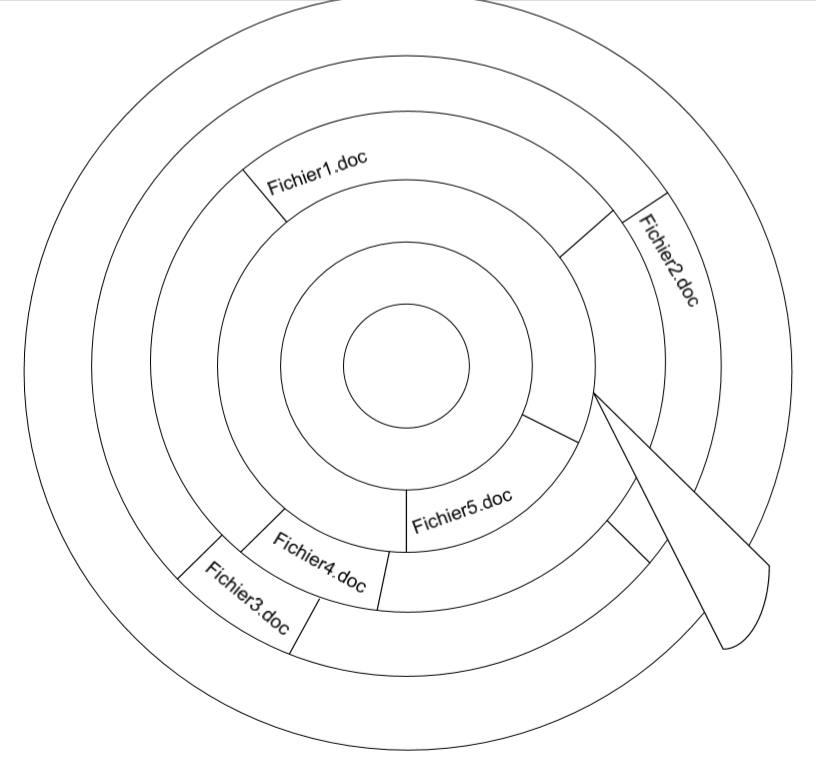
\includegraphics[scale=0.4]{info-stockageContigu}\caption{Stockage contigu des fichiers}\label{fig:stockageContigu}}
Les fichiers sont lus de manière contiguë : on commence par le début et on le lit progressivement. On comprend donc que la disposition telle qu'affichée sur la figure \textbf{\ref{fig:stockageContigu}} tient son sens : le bras de lecture (sur la droite de la figure) lit le fichier de manière séquentielle et contiguë. C'est une manière qui présente des bonnes performance en temps pour des fichiers accédés en mode séquentiel, étant donnés les déplacements limités du bras. De plus, l'adressage logique du programme est facilement convertible en adresse physique car l'adressage physique se fait par rapport à un point de référence, l'adresse du début du fichier sur disque. Cette manière de stocker possède néanmoins des désavantages, dont la possibilité de se transformer en gruyère par exemple (détaillé ci-dessous), et l'inflexibilité de la taille des fichiers. \\
\\
Supposons un instant que le disque dur ait été construit avec les fichiers répartis de manière contiguë. Si on efface, et crée des fichiers de manière récurrente et qu'on laisse une répartition contiguë, c'est plus difficile d'optimiser la répartition d'espace. En effet, si on supprime un fichier et qu'on veuille installer un autre fichier à son emplacement. Comme il sera très rarement de la même taille, on aura soit un fichier trop gros pour l'espace et donc non-plaçable dedans, soit trop petit et donc créer un trou (d'où l'appellation "gruyère"...).  \\
\\
Un autre désavantage est qu'il est impossible de faire grandir un fichier à moins de le déplacer dans un endroit suffisamment grand, laissant derrière lui un espace vide qui, comme on l'a vu avec le gruyère, ne sera pas complété de manière optimale.
\subsubsection{Stockage en liste liée}
\wrap{13}{r}{0.4}{
\vspace{-0.5cm}
\centering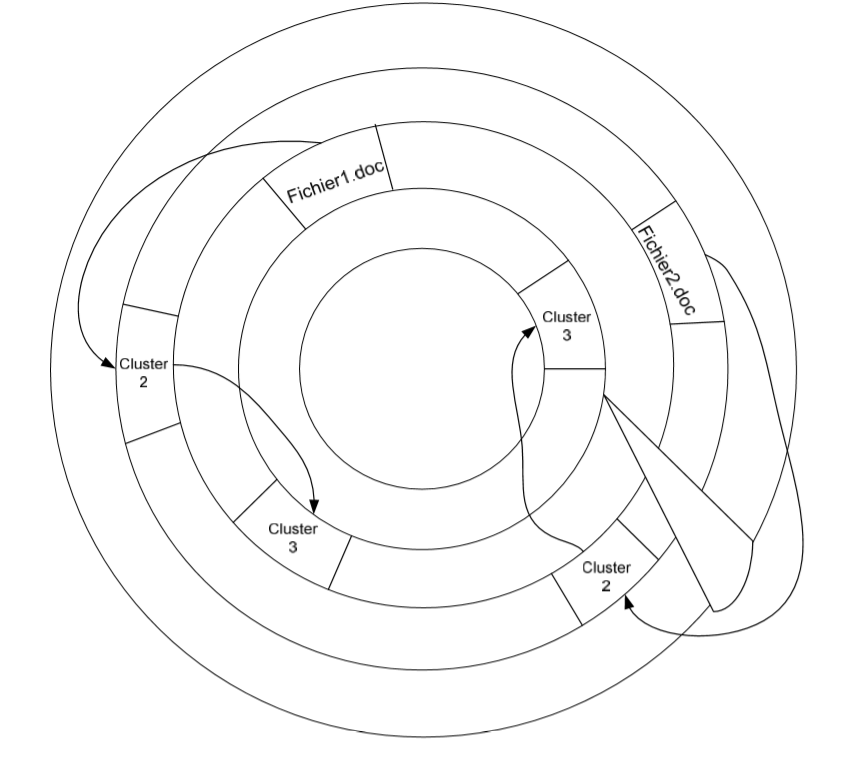
\includegraphics[scale=0.4]{info-stockageListeLiee}
\caption{Stockage en liste liée.}
\label{fig:stockageListeLiee}}
 Une autre manière est la répartition éclatée via le stockage de fichiers en liste liée. La liste liée consiste à associer un fichier à des pointeurs : chaque \textbf{fichier} se trouve maintenant \textbf{éclaté} sur le disque dur. Il est impératif de concevoir dès lors des algorithmes d'accès physiques afin de relire le fichier et de le reconstituer dans son intégralité. L'avantage principal de la liste liée est la possibilité de grossissement et le rapetissement de fichiers, étant donné que chaque bout de fichier envoie vers le suivant. Cette manière de reconstruire un fichier suivant des agrégats est optimale parce que pour supprimer/ajouter quelque chose au fichier, on n'a qu'à ajouter/supprimer l'agrégat en question et ajuster le pointeur (\textbf{cluster}) en fonction. \\
  \\
Les désavantages là sont d'une part les grandes distances à parcourir par le bras de tête, ce qui pose un problème pour les accès directs (RAM). La liste liée s'adapte en effet assez bien pour les accès en séquentiel (mémoires d'archivage par exemple). D'autre part un pointeur endommagé entraîne la perte du fichier. 


\subsubsection{Stockage selon table indexée}
\wrap{17}{r}{0.4}{
\vspace{-0.5cm}
\centering
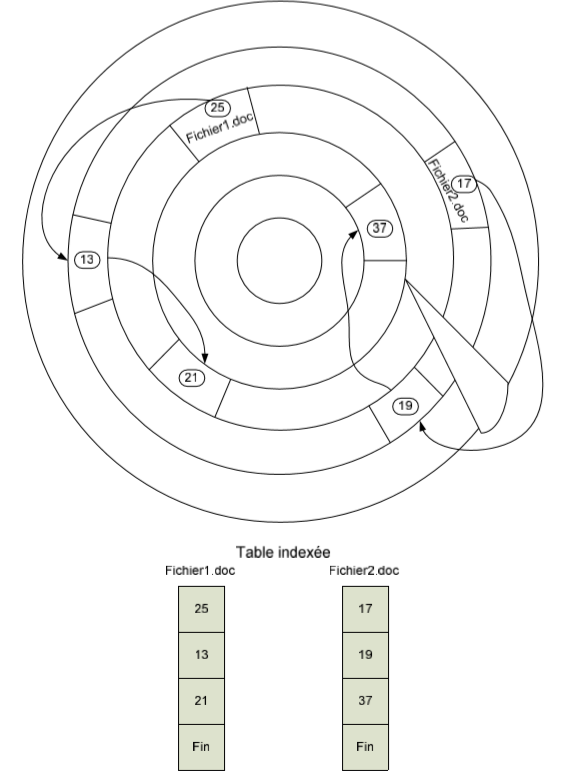
\includegraphics[scale=0.5]{info-stockageIndexee}
\caption{Stockage selon table indexée}
\label{fig:stockageTableIndexee}}
 Une troisième manière de stocker les fichiers est via \textbf{une table indexée}, contenant toutes les adresses de tous les clusters de notre fichier. C'est de loin la meilleure solution pour des accès logiques de type direct ou aléatoire (RAM) car il suffit de localiser l'index dans la table pour récupérer l'adresse physique (sous forme de numéro d'agrégat) où l'information désirée se trouve. La corruption d'une partie de la table est moins grave que pour un stockage en liste liée, qui pour rappel, entraînait la perte du fichier, mais la présence de la table pose néanmoins problème parce qu'elle prend un certain temps à parcourir, vu que c'est fait entrée par entrée, et parce que c'est quand même quelque chose qu'il faut stocker : la table indexée occupe un espace \textbf{incompressible} du disque car elle stocke toute l'information sur son contenu.\\
 \\
 Elle est vraiment absolument ruina parce que \textbf{tant que la table indexée n'a pas changé d'avis sur une information}, c'est-à-dire que l'information n'a pas été réécrite, \textbf{elle peut toujours permettre de la récupérer}. Autrement dit même si on supprime un morceau de fichier par mégarde, tant qu'il n'y a rien été réécrit dessus des logiciels spécialisés permettraient de récupérer l'information. Par contre si on perd la table indexée on perd toutes les données. On comprend que quand on formate un disque en fait on ne "supprime" pas les données mais on efface le contenu de la table indexée. Tous les fichiers sont encore là, ils sont juste inaccessibles et sont prêts à être remplacés par des nouveaux qui seront adressables à partir de la table indexée. Si par malheur on perd la table indexée, il y a aussi moyen, au travers de logiciels spécialisés, de la reconstruire.

\subsection{Stockage logique des fichiers}

\subsubsection{Gestion du répertoire}
Le répertoire est quelque chose qu'on ne comprend pas très bien : déjà ce n'est pas un emplacement physique. Même si on le bouge avec la souris, ça n'a rien de physique. Le répertoire est un système de \textbf{dénomination}, c'est le préfixe qu'on ajoute à un fichier pour en assurer l'unicité de l'identification et lui permettre le rattachement à une famille de fichiers aux caractéristiques communes. Le répertoire est par ailleurs aussi un fichier en tant que tel, et par exemple quand on clique dessus ça nous affiche tous les fichiers qui se cachent derrière le nom du répertoire.\\
\\
L'utilité des répertoires est bien plus multiple que ce que l'on pense : déplacement en bloc d'un répertoire vers un autre, réutilisation d'un même nom de fichier dans plusieurs répertoires, définition comme de droits d'accès, regroupement selon des critères tels que l'utilisateur, application, domaine d'activités, ou même critère laissé au choix de l'utilisateur. \\
\\
Pour finir, tout répertoire est attaché au \textit{root directory}, qui forme lui le point de départ d'une succession de répertoires associés aux mémoires secondaires. Comment intégrer la gestion de l'espace physique sur disque à la structure logique en répertoires ? C'est la section qui suit.

\subsubsection{Répertoires et FAT}
La gestion de fichier via FAT, "File Allocation table", est une forme de liste liée (cf section précédente) qui utilise une table indexée. L'idée est la suivante : à chaque disque correspond une table d'allocation qui reprend l'état de chaque unité d'allocation, et contient autant d'entrées qu'il y a d'agrégats (clusters) sur le disque. Donc chaque unité d'allocation indique l'état d'un agrégat, indiquant soit le numéro de l'agrégat suivant, soit qu'il s'agit de la fin du fichier, soit "0" si l'agrégat est inoccupé. À cette table viennent s'ajouter d'autres informations utiles à la reconstitution de fichiers, dont la plus importante est le \textbf{numéro de cluster du début de fichier}.
\subsubsection{Système de gestion NTFS (Windows NT)}
Ce système, NT \textit{File System}, n'est plus basé sur la FAT qui renseigne sur la succession des agrégats mais sur des informations contenues dans une MFT (\textit{Master File Index}), une liste d'entrée de 1Ko pour chaque fichier. Chaque entrée de la MFT constitue un "objet" comme dans le sens de l'orienté objet : décrit par des attributs, tels que l'emplacement des agrégats par exemple. La sécurisation des fichiers et répertoires est assurée par des permissions d'accès telles que \textbf{R} (\textit{read}), \textbf{W} (\textit{write}), \textbf{X} (\textit{execute}), etc.\\
\\
La fiabilité du système NTFS est assurée par la présence dans la MFT d'un journal des opérations sur ses structures, permettant notamment sa reconstruction suite à un crash du système, affectant le disque dur. Précisons enfin que les petits fichiers sont appréciés par la MFT parce leurs données peuvent être contenues dans le même agrégat que leur description respective.

\subsubsection{Stockage des fichiers dans Unix}
Unix utilise un système de stockage de fichiers basé sur une table indexée. À chaque répertoire est associé un fichier contenant une liste de noms de fichiers auxquels sont associés des pointeurs vers une table d'index nommée "i-node", qui contient toute l'information nécessaire à l'utilisation d'un fichier et contient un ensemble d'attributs et de pointeurs si une seule table ne suffit pas à l'encodage de tous les attributs. Il y aura donc pointage vers des autres i-nodes qui pointent eux aussi vers d'autres i-nodes etc. mais toujours de manière à avoir les données à la fin (figure \textbf{\ref{fig:inode}} ). 
\begin{figure}[h!]
\centering
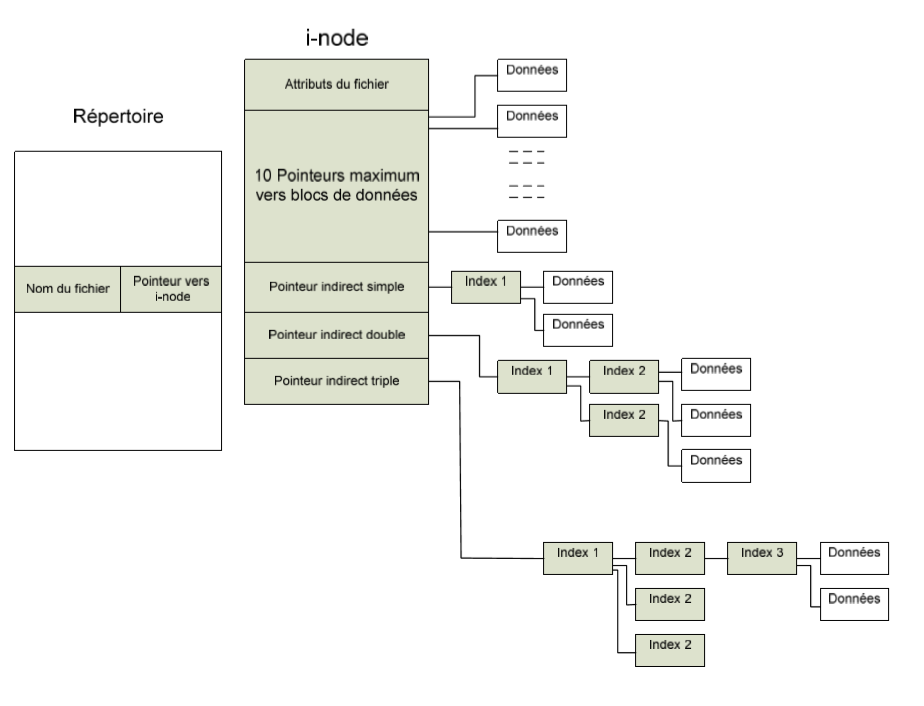
\includegraphics[scale=0.5]{info-i-node}
\caption{Stockage logique des fichiers en i-node. Stockage physique correspondant : stockage selon table indexée.}
\label{fig:inode}
\end{figure}
On accède donc aux données mais via des indirections qui évitent le fait d'avoir des tables indexées trop grosses, qui peuvent par ailleurs dépasser la taille du fichier lui-même si trop conséquente.

\subsection{Structuration logique des fichiers}
\subsubsection{Généralités}
Fondamentalement, un fichier est une collection séquentielle d'octets contenus dans une suite dispersée d'agrégats (clusters) et présentée au programme sous une forme contiguë via le gestionnaire de fichiers. Par contre vu du disque dur, un fichier est réduit à une suite "éclatée" d'agrégats à prélever sous forme de "blocs". Vu de l'OS, un fichier est donc un espace de longueur donnée, éparpillé sur le disque. Chaque OS gère cet espace à sa convenance  \textbf{sans s'occuper du contenu logique des fichiers}. Le gestionnaire de fichiers de l'OS se limite à allouer cet espace à un programme en exécution (un processus) en vérifiant que ce-dernier soit habilité à y accéder. Il commence alors à répondre aux sollicitations du processus, consistant à lire ou écrire un certain nombre d'octets en précisant l'emplacement relatif du fichier. Le gestionnaire vérifie alors que le processus demandeur ne déborde pas de l'espace qui lui est alloué.\\
\\
\subsubsection{Organisation du contenu}
L'OS ne voit pas le contenu des fichiers et s'en fout royalement, il ne s'occupe que de fournir aux programmes un accès neutre au contenu des fichiers. Cet accès est souvent \textbf{séquentiel}, c'est-à-dire que le fichier est parcouru progressivement du premier octet jusqu'au dernier. L'ajout ou retrait d'un octet qui n'est pas à l'extrémité finale demande la réécriture complète du fichier par un programme de traitement de fichier. Celui-ci demande l'accès au fichier via le gestionnaire de fichiers, en précisant le nombre d'octets à lire ou le nombre d'octets à écrire ainsi que le point d'arrivée de l'opération précédente.


\chapter{Les réseaux}
\section{Introduction, contexte}
Les réseaux, c'est important. Tous les processeurs peuvent communiquer entre eux par des réseaux : des 1 et des 0 on peut les envoyer via des fils de courant, des fibres optiques, etc. Les réseaux informatiques mettent en place des communications très simples, et c'est ça qui forge les révolutions actuelles, : la transmission simple des informations.\\
\\
Avant, le réseau dominant était la téléphonie, et il fallait réserver tout un canal entre les interlocuteurs et il faut que la transmission soit parfaite. C'est l'art de la \textbf{commutation} de circuit : réserver des lignes qui sont là pour la transmission d'information
\subsection{Dématérialisation des supports}
L'essentiel des réseaux se base sur la notion d'échange. Au cours de l'histoire, le besoin d'échange a en effet demeuré alors que le médiateur n'a cessé de se métamorphoser : on est passé du troc, nécessitant affiliation et contact physique entre les intervenants, successivement à la monnaie physique et les transitions bancaires en ligne. L'informatique a grandement accompagné cette dématérialisation au travers des réseaux.
\subsection{Digital vs Analogique}
\begin{itemize}
\item Un signal \textbf{analogique} est un signal qui varie de manière continue dans le temps.
\item Un signal \textbf{digital} est un signal discrétisé en binaire.
\end{itemize}
Pour les raisons qu'on vient de voir les 5 chapitres précédents, l'information est plus facilement traitée quand elle est en binaire, et il faut donc prendre du temps pour traduire les signaux, pour les certains qui sont analogiques, en signaux digitaux. Prenons l'exemple du téléphone, les extrémités sont des signaux analogiques parce que la bouche comme l'oreille, l'information est reçue/envoyée de manière continue dans le temps.
\section{Types de support physique}
\subsection{À propos du multiplexage}
Les supports assurent la transmission matérielle des signaux. Ils peuvent assurer le passage simultané de signaux, c'est ce qu'on appelle le \textbf{multiplexage}. Ce mécanisme est assuré par un multiplexeur qui groupe les signaux à une extrémité et un démultiplexeur qui les dégroupe à l'autre extrémité.\\
\\
Le multiplexage peut être de différents types : temporel, spatial, ou statistique.
\begin{itemize}
\item Un multiplexage \underline{temporel} consiste à déterminer des intervalles de temps sur un support rapide de manière à pouvoir les affecter successivement  des franges de données (bits, octets) en provenance de supports au débit moindre. Par exemple, une ligne à 2 Mb/s multiplexe 30 canaux à 64 kb/s (une partie est affectée à la matérialisation des intervalles de temps et à la signalisation).
\item  Un multiplexage \underline{spatial}, ou \underline{en fréquence},  consiste à superposer plusieurs fréquences sur un même support et à moduler chacune de ces fréquences en fonction du signal transporté. Ce type de multiplexage est très utilisé pour les grandes transmissions par fibres optiques, en superposant les différentes longueurs d'onde pour multiplier le nombre de canaux.
\end{itemize}
 
\subsection{À propos des transmissions}
Les transmissions peuvent être de différents types, avec deux classifications supplémentaires à la fin :
\begin{itemize}
\item Transmission simplex ou unidirectionnelle : ne permet que l'envoi dans une direction. Exemple : une sonde.
\item Transmission semi-duplex ou bidirectionnelle : permet l'envoi de signaux dans les deux sens mais de manière alternée et jamais simultanée. Exemple : les \textit{talkie-walkie}.
\item  Transmission duplex : permet l'envoi des signaux dans les deux sens simultanément, comme c'est le cas du téléphone. Les débits de part et d'autre peuvent néanmoins être différents.
\item Point à point : quand une information circule entre 2 points et part d'un point A en étant destinée à un point B. C'est le cas d'un mail, ou d'une conversation téléphonique : une information arrive à un endroit précis en suivant un chemin.
\item Multipoint : l'information est diffusée à tous ceux qui peuvent/veulent la recevoir.
\end{itemize}
Une communication par téléphone est donc duplex multipoint, étant facilement accessible par les autres ou espionnée.\\
\\
Il y a 3 supports principaux de communication : le courant électrique, les ondes électromagnétiques, et l'optique (à travers les fibres optiques) ; tout est bon pour véhiculer des 1 et des 0. L'antenne WI-FI c'est par onde électromagnétique par exemple. 
Lors d'une communication par fils on se doit de protéger le signal, c'est pourquoi on voit des fils torsadés. Le câble coaxial est plus fiable et rapide et permet une distance de transmission plus grande que les fils torsadés. La fibre optique elle, a un grand avantage dans sa finesse (plus fine qu'un cheveux) et sa rigidité au bruit. Mais tous ces modes sont détaillés dans les sections qui suivent.

\subsection{Ondes électromagnétiques}
Les ondes ont une fréquence/longueur d'onde. L'essentiel de la communication se fait dans les ondes \textbf{radio} ($\nu = 30$kHz $\rightarrow 300$GHz). Les ondes EM sont un "bien commun" parce qu'elles sont partageables librement, personne ne les \textit{possède}, mais il y a des opérateurs qui achètent des fréquences pour y véhiculer leurs infos.\\
\\
Les fréquences basses peuvent franchir plus d'obstacles, donc on peut voir sur le spectre électromagnétique que WI-FI est plus robuste que Bluetooth.\\
\\
Pour transmettre des 0 et des 1 via une onde sinusoïdale, on utilise ses caractéristiques qui sont l'amplitude, le déphasage, et la fréquence. Là aussi il y a des études pour essayer d'optimiser le transport d'informations via les ondes électromagnétiques.
\subsection{Télécommunication --- commutateurs, autocommutateurs, et Internet}
Histoire de la téléphonie ! Une conversation téléphonique consistait en un transfert d'informations via un circuit qui lie les deux interlocuteurs. Ce circuit s'appelle un "commutateur" : chaque correspondant est relié par une ligne ou circuit à une installation centrale, où un opérateur établit à la demande une connexion par un circuit rejoignant le correspondant souhaité, et ce pour une durée limitée. Le circuit est le \textbf{même} pour un utilisateur, ce qui explique que les informations vont bien arriver dans le bon ordre. On peut voir ça dans la figure \textbf{\ref{fig:commutateurs}}. La commutation était faite au début manuellement, et ça a commencé par après à devenir automatique (autocommutateurs). Par après, la progression de la télécommunication s'est traduite par l'augmentation du nombre de lignes, de la qualité des transmissions, du débit entre circuits (utilisation de la fibre optique), disponibilité et débit des réseaux mobiles, ...\\
\begin{figure}[h!]
\centering
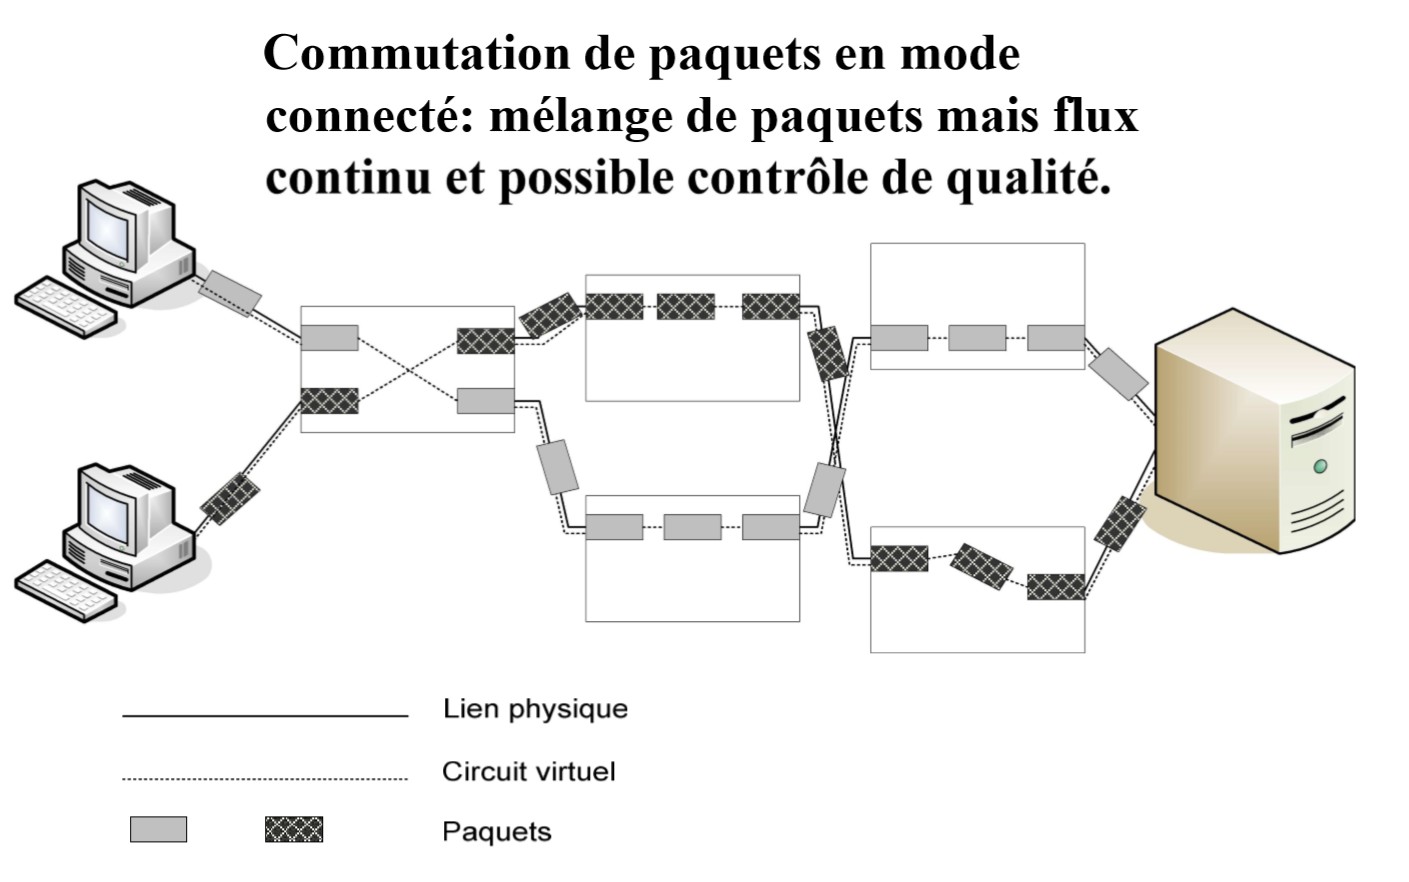
\includegraphics[width=0.7\textwidth]{info-paquetsCommutateur}
\caption{Réseau téléphonique : les commutateurs. Chaque élément de conversation passe par le même chemin.}
\label{fig:commutateurs}
\end{figure}
Par contre, pour véhiculer des messages, par exemple des textes, on remarque qu'il n'est pas nécessaire de consacrer une ligne. Une première idée est par exemple de couper un message en paquets, et de faire transférer les messages par multiplexage sur Internet. Mais les paquets pourraient très bien arriver dans un mauvais ordre, étant donné que sur Internet, les informations ne suivent pas le même circuit : tous les paquets prennent des chemins différents, dépendant de la saturation des chemins. Pourtant, la qualité d'envoi des information est \textbf{très exigeante} !\\
\\
On essaye dès lors de retrouver les exigences de l'époque de la téléphonie : on veut retrouver les données dans le même ordre, notamment. Alors on décide comme pour les téléphones que tous les paquets de même types vont parcourir le même chemin. Par contre, une nouveauté intervient parce que les données peuvent se mélanger au long d'un chemin, c'est \textbf{ça} la nouveauté d'Internet. Internet s'est voulu dès le départ totalement égalitaire et démocratique : un routeur ne connaît pas le contenu d'un paquet. Les paquets sont aiguillés en fonction de leur destination mais pas de leur contenu : \textbf{aucun paquet n'a priorité sur un autre}. Par contre dans le monde d'aujourd'hui on commence à faire payer la priorité des paquets. Comment privilégier un service ? C'est en regardant les chemins et en envoyant tous les paquet sur un chemin peu fréquenté par exemple.

\section{Réseaux LAN (Local Area Network)}
On entre maintenant dans le monde des petits réseaux, pour lesquels on utilise la terminologie d'Ethernet pour symboliser la plateforme de connexion entre machines. Une machine a, dès sa création, une adresse Ethernet, l'adresse M.A.C., qui lui procure une identification aux yeux du réseau local (c'est le rôle de la carte réseau). Dans le monde des petits réseaux, il y a 3 modes de connexion : le bus

\subsection{Bus}
L'idée est de mettre un fil et de connecter les ordinateurs via des fils. Avec des prises Ethernet on connectait les ordinateurs entre eux. Le système d'exploitation repérait le réseau, l'adresse MAC et faisait tout pour que ça se passe bien, mais le problème est qu'Ethernet n'est pas fiable. 
\begin{itemize}
\item Le premier problème est le risque de collisions, parce que tous les ordinateurs passent par le même bus. Il y avait un protocole de détection et correction de collisions.
\item Le deuxième problème est qu'Ethernet est là en multipoint (rien n'empêche l'information de parvenir à tous les ordinateurs). Si un ordinateur envoie un message à un autre, c'est tous les ordinateurs qui peuvent le percevoir . Ce qui se passe dans Ethernet quand il est en mode Bus, c'est que si un ordinateur est défaillant (sa carte réseau est défaillante) et qu'il reçoit une information, alors l'information est \textbf{perdue}.
\end{itemize}
C'est pour ça qu'on laisse tomber le mode Bus.
\begin{figure}[h!]
\centering
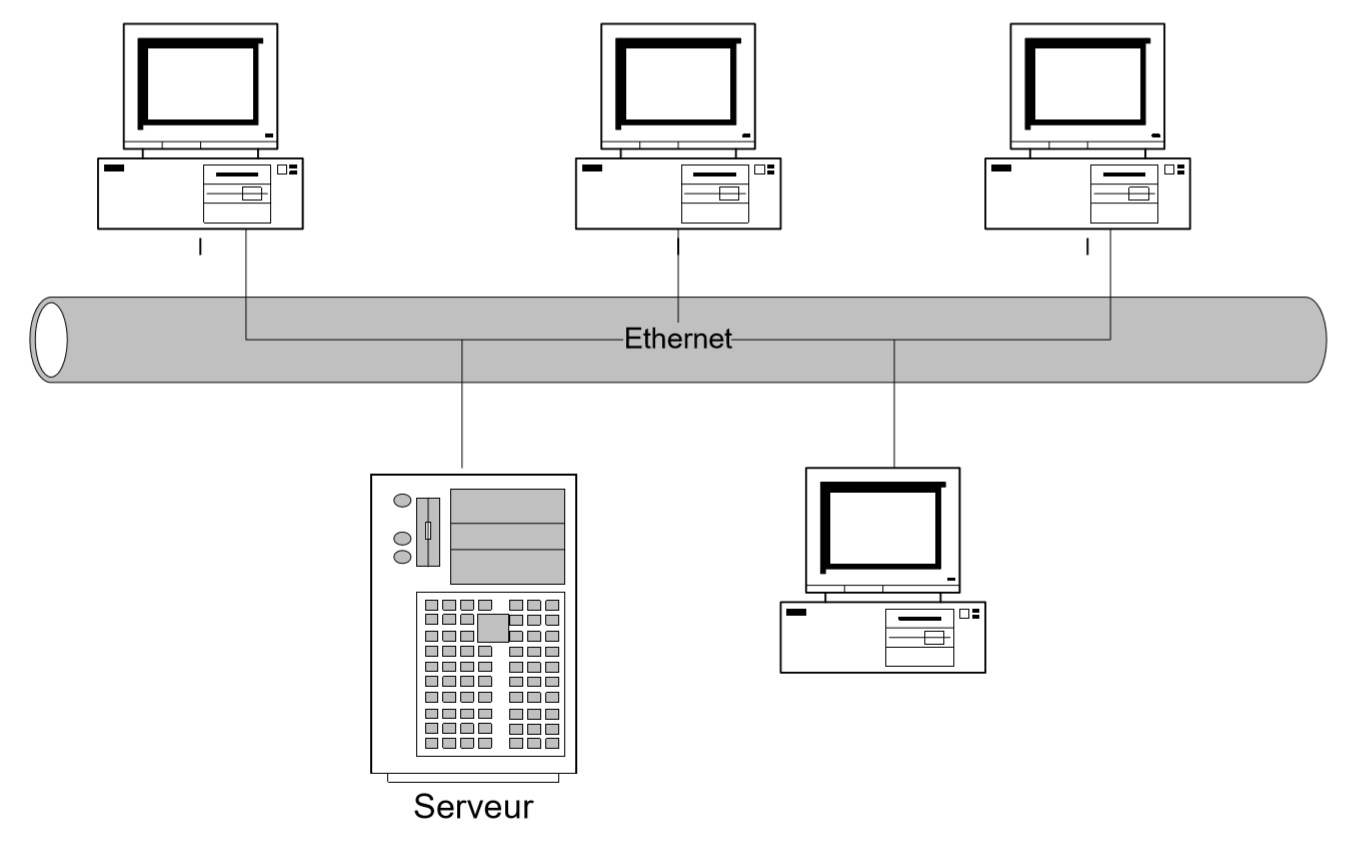
\includegraphics[scale=0.5]{info-bus}
\caption{Illustration d'une connexion Ethernet en mode Bus}
\label{fig:bus}
\end{figure}
\subsection{En étoile}
\wrap{11}{r}{0.3}{\centering
\vspace{-0.5cm} 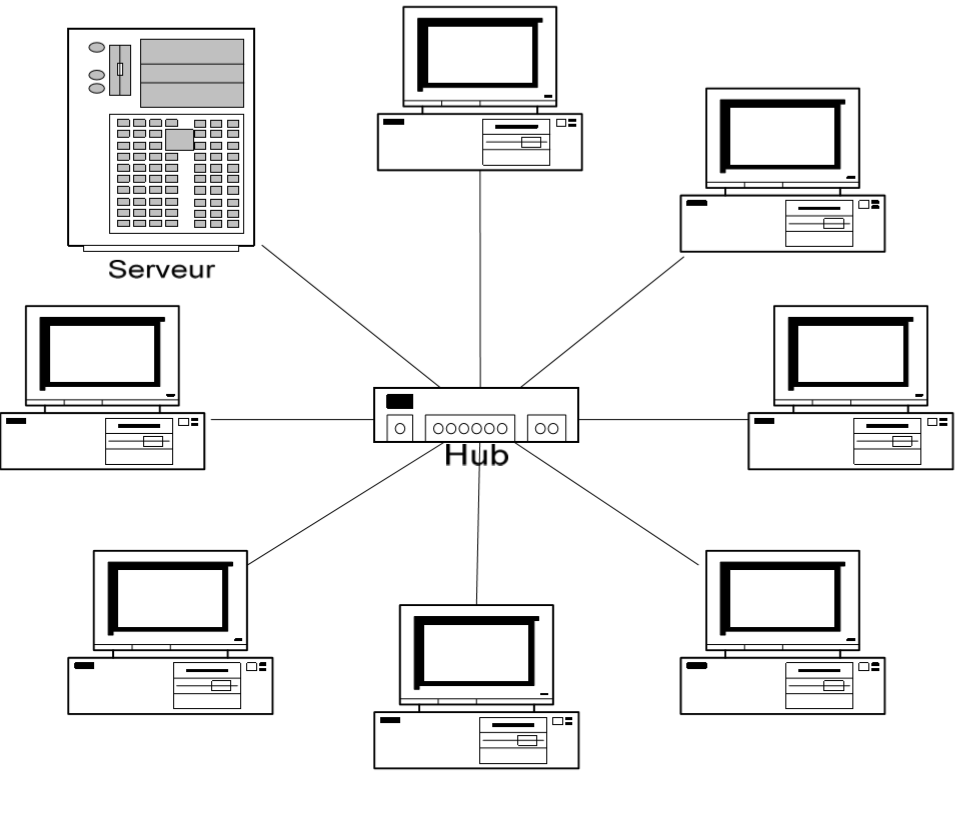
\includegraphics[scale=0.25]{info-etoile}
\caption{Connexion Ethernet en étoile via un HUB.}}
Tout est autour d'un "hub", et c'est beaucoup plus fiable au niveau des collisions et de la défaillance d'une machine, vu que le message ne passe pas forcément partout. On n'est en effet plus en multipoint mais c'est le hub qui redirige un ordinateur vers un autre quand celui-ci veut envoyer un message : l'ordinateur envoie un message et le hub le transmet à un ordinateur précis, sans diffuser le message à tout le monde. Le WIFI est simplement le protocole Ethernet à la sauce électromagnétique.

\section{Protocoles de communication}
\subsection{Modèle OSI}
Quand un ordinateur veut communiquer à un autre : un échange de mails par exemple. Ce mail il a du faire pas mal de choses pour pouvoir transiter entre nous et le destinataire. Et s'il a transité c'est qu'il doit y avoir un support physique. Si on est dans le cas d'un réseau Internet, le mail est envoyé à un routeur, puis à un autre, etc. jusqu'à arriver au destinataire. Mais le mail est divisé en paquets ! Donc il faut s'assurer que les paquets soient bien reçus et possibles à remettre dans le bon ordre. Internet est un protocole en \underline{7 couches}.\\
\\
Chaque couche va s'occuper d'une partie de la communication. On a les mêmes couches du côté expéditeur et du côté destinataire, et seules les mêmes couches se comprennent ! Par exemple, si une couche décide de couper l'information en paquets, seule son équivalente de l'autre côté ne comprend cette notion de paquet. Les couches se suivent en se passant la main et s'organisent vis-à-vis de l'information de la manière qui suit : on descend en ajoutant de l'information via les couches du dessus puis les couches du dessous, chaque information ne pouvant être comprise que par son alter-égo, et cet alter égo lit l'information la plus récemment mise, donc il traite l'information du bas des couches vers le haut\footnote{C'est normal vu que la première info que le destinataire voit c'est celle de la dernière couche de l'expéditeur, celle du bas, qui ne peut être comprise par la couche du bas du destinataire.}.
\begin{figure}[h!]
\centering
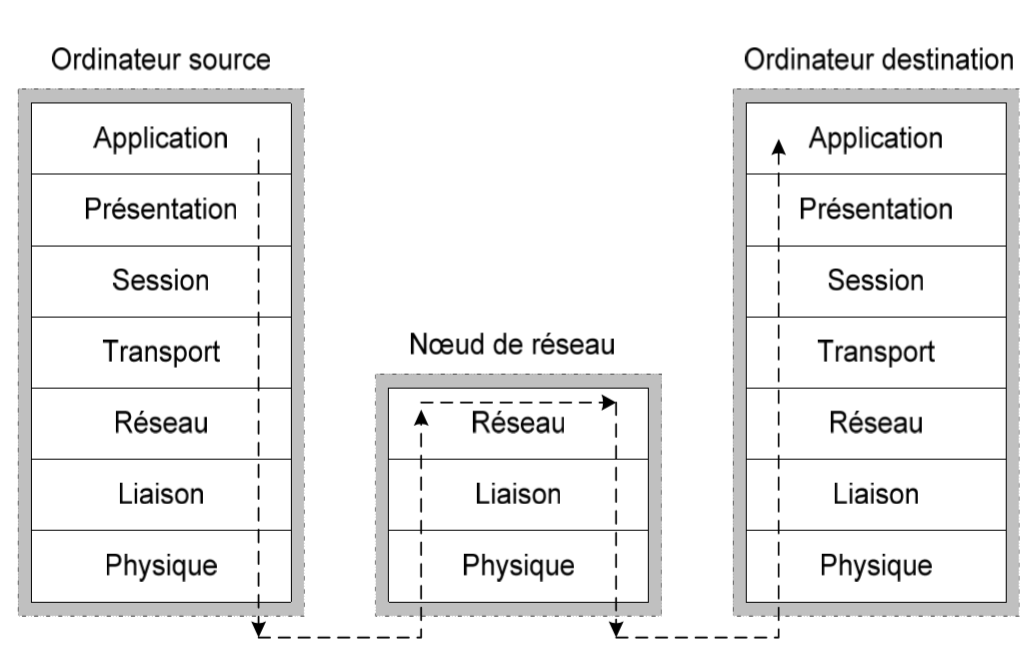
\includegraphics[scale=0.4]{info-osi}
\caption{Modèle OSI}.
\label{fig:osi}
\end{figure}
On peut voir que si l'on veut envoyer un mail, ça part de la première couche en haut à gauche et ça arrive à la dernière couche en haut à droite, mais ça a parcouru tout un chemin avant. Que font les couches du milieu ?
\subsubsection{Noeud de réseau}
Quand on a conçu Internet initialement, on l'a conçu en lest 7 couches de la figure \textbf{\ref{fig:osi}}, avec au milieu le \textbf{routeur}, qui ne connait PAS la nature de l'information, il est là juste pour s'assurer que "le paquet" transite bien. Les 7 couches, elles, doivent savoir quel est le type d'informations qui transite.
\subsubsection{Les 7 couches}
Quand on présente Internet on présente les 7 couches parce que c'est théoriquement ce que ça doit être.
\begin{enumerate}
\item Physique : comment on transfère des 1 et des 0
\item La couche liaison : celle qui fait le lien entre Internet et Ethernet. Par exemple, on est sur notre ordinateur et on veut envoyer un mail, bah on est quand même sur notre ordinateur, donc on est sur Ethernet. Dès lors qu'on est sur Ethernet, notre message doit être découpé en paquets.
\item Couche réseau : celle qui fait le routage. On envoie notre mail aux États-Unis mais il est possible que le premier routeur qu'on rencontre est un routeur en France, pas aux USA. Et c'est pour ça qu'on fait le routage : le routeur en France regarde le paquet, regarde où est ce qu'il doit aller, regarde dans la table de routage pour regarder le chemin le plus efficace sans doute, et envoie le paquet vers un autre routeur. Jusqu'à arriver à un moment au routeur final : le routeur du réseau de notre destinataire final aux USA. Ce routeur dira "OK on est sur le réseau de notre destinataire", et après ça il le distribuera sur l'Ethernet du destinataire etc. En tout cas on est sur le réseau du destinataire mais il faut que le paquet arrive chez la machine du destinataire et surtout, qu'on remette les paquets dans l'ordre.
\item Transport : détection des erreurs à l'arrivée. Comment on fait ? Les bits de vérification vus en début de chapitre 1. Ce sont des protocoles de vérification.
\item Session : ouverture et synchronisation du dialogue.
\item Présentation : ce qui permet par exemple de mettre notre e-mail sous forme binaire.
\item Application : celle qui dit ce qu'on veut faire sur Internet, parmi les listes de protocoles ("mail", "http", "FTP" (file transfer protocol)...).
\end{enumerate}
Depuis, on a simplifié ce protocole en 4 couches. Il faut en tout cas bien comprendre que les protocoles doivent se parler entre eux, et que Internet parle à Ethernet : dès que les paquets arrivent à destination, Ethernet s'en occupe.
\subsection{Protocole Ethernet}
On vient de voir comment fonctionne Internet, maintenant regardons comment fonctionne Ethernet. On a déjà vu Bus \& étoile. De nos jours, on parle d'Ethernet Gbits. Chaque poste a une carte Ethernet (adresse MAC), et lors de la réception d'un paquet la machine vérifie si le paquet est bien destiné à son adresse. La plupart des utilisations d'un protocole Ethernet se fait à partir de protocoles Internet. En effet, l'Internet étant beaucoup plus global, la circulation se fait d'abord entre routeurs, et une fois arrivé au bon routeur, on entre en Ethernet.
\subsection{Le sans-fil}
Le WIFI est une fréquence d'environ 2.4 GHz, et il y a peu de risque de collsions.
\subsection{Internet et TCP/IP}
L'ordinateur a une adresse MAC \textbf{définitive}, qui lui permet de s'identifier sur l'Ethernet. Si on veut se connecter à Internet il lui faut aussi une adresse pour s'identifier sur Internet, mais elle ne sera pas physique parce qu'elle dépend d'où on est, de la connexion en question, etc. Quand on veut se connecter à Internet, on fait d'abord appel à un opérateur et ce-dernier va nous allouer des adresses Internet (fictives et non-stables) pour pouvoir s'y identifier. L'adresse qu'on reçoit n'est pas physique et pas stable ! L'adresse physique stable est chez l'opérateur, sur un serveur, qui reçoit tous les message qui nous est destiné.\\
\\
Comment on connaît ces adresses Internet ? C'est le bordel. Internet doit connaître les adresses fixes, et il faut donc voir comment on va distribuer les adresses Internet. Cette décision conditionne considérablement le fonctionnement d'Internet. La décision a été d'adresser ça sur 32 bits, ce qui donne un nombre de $2^{32} \approx 4$Md adresses, un peu trop faible.
\subsubsection{Adresse IP}
L'adresse internet s'appelle l'adresse IP, et varie en style selon les organisations, selon des classes :
\begin{itemize}
\item[A] Organisations de très grande taille, avec une adresse station sur 24 bits. On commence avec un bit de 0, et donc possibilité de créer $2^7$ réseaux (1 bit + 7 bits + 24 bits = 32 bits).
\item[B] Adresse sur 16 bits (universités par exemple), et on commence par un 1 et un 0, donc possibilité de créer $2^{14}$ réseaux.
\item[C] Pour les petites organisations, 8 bits.
\end{itemize}
On écrit une adresse IP comme ça : (8 bits).(8 bits).(8 bits), donc par exemple 191.181.180.119, et ça ça va nous définir l'appartenance à une classe. Par contre comme c'est dur à retenir, on va préférer une adresse symbolique comme "ulb.ac.be" : ce sont les noms de domaine.

\subsection{Protocole hiérarchique}
\begin{enumerate}
\item Au niveau de l'application, on fixe l'adresse IP du destinataire. On cherche ça dans le DNS.
\item Protocole TCP :  on fait les paquets, on établit la session, on envoie les paquets, on s'assure que tous les paquets sont reçus dans le bon ordre (et on corrige éventuellement).
\item Au niveau IP, on s'occupe du routage.
\end{enumerate}
\end{document}
